% --- LaTeX Lecture Notes Template - S. Venkatraman ---

% --- Set document class and font size ---

\documentclass[letterpaper, 12pt]{article}


% --- Package imports ---

% Extended set of colors
\usepackage[dvipsnames]{xcolor}

\usepackage{
  amsmath, amsthm, amssymb, mathtools, dsfont, units,          % Math typesetting
  graphicx, wrapfig, subfig, float,                            % Figures and graphics formatting
  listings, color, inconsolata, pythonhighlight,               % Code formatting
  fancyhdr, sectsty, hyperref, enumerate, enumitem, framed }   % Headers/footers, section fonts, links, lists

% lipsum is just for generating placeholder text and can be removed
\usepackage{hyperref, lipsum} 
% \usepackage{bm}
% \usepackage{subfig}

% --- Fonts ---

\usepackage{newpxtext, newpxmath, inconsolata}
\usepackage{amsfonts}
\usepackage{pgfplots}
\pgfplotsset{compat=1.12}
\usepackage{tkz-fct}
\usepackage{svg}
\usepackage{tikz}
\usepackage{tikz-cd}
\usepackage{lipsum}
\usepackage{enumitem}
\usepackage[title]{appendix}
% \usepackage[toc,page]{appxendix}
\usepackage[utf8]{inputenc}
\usepackage{multicol}
\usepackage{multirow}
\usepackage{booktabs}

\usepackage{minted}  % code highlighting
% \usepackage[finalizecache,cachedir=.]{minted}
% \usepackage[frozencache,cachedir=.]{minted}

\DeclareUnicodeCharacter{3BC}{$\pi$}
\DeclareUnicodeCharacter{3C0}{$\pi$}

\usepackage[most]{tcolorbox}
\newtcolorbox{myquote}[1][]{%
  colback=black!5,
  colframe=black!5,
  notitle,
  sharp corners,
  % borderline west={2pt}{0pt}{red!80!black},
  enhanced,
  breakable,
}

\renewcommand*\pod[1]{%
  \allowbreak
  \mathchoice
    {\mkern 18mu}%
    {\mkern  8mu}%
    {\mkern  6mu}% "6mu" matches the space *after* the word "mod"
    {\mkern  6mu}%
  (#1)%
}

% --- Page layout settings ---

% Set page margins
\usepackage[left=1.35in, right=1.35in, top=1.0in, bottom=.9in, headsep=.2in, footskip=0.35in]{geometry}

% Anchor footnotes to the bottom of the page
\usepackage[bottom]{footmisc}

% Set line spacing
\renewcommand{\baselinestretch}{1.2}

% Set spacing between paragraphs
\setlength{\parskip}{1.3mm}

% Allow multi-line equations to break onto the next page
\allowdisplaybreaks

% --- Page formatting settings ---

% Set image captions to be italicized
\usepackage[font={it,footnotesize}]{caption}

% Set link colors for labeled items (blue), citations (red), URLs (orange)
\hypersetup{colorlinks=true, linkcolor=RoyalBlue, citecolor=RedOrange, urlcolor=ForestGreen}

% Set font size for section titles (\large) and subtitles (\normalsize) 
\usepackage{titlesec}
% \titleformat{\section}{\large\bfseries}{{\fontsize{19}{19}\selectfont\textreferencemark}\;\; }{0em}{}
\titleformat{\section}{\large\bfseries}{\thesection\;\;\;}{0em}{}
\titleformat{\subsection}{\normalsize\bfseries\selectfont}{\thesubsection\;\;\;}{0em}{}

% Enumerated/bulleted lists: make numbers/bullets flush left
%\setlist[enumerate]{wide=2pt, leftmargin=16pt, labelwidth=0pt}
\setlist[itemize]{wide=0pt, leftmargin=16pt, labelwidth=10pt, align=left}

% --- Table of contents settings ---

\usepackage[subfigure]{tocloft}

% Reduce spacing between sections in table of contents
\setlength{\cftbeforesecskip}{.9ex}

% Remove indentation for sections
\cftsetindents{section}{0em}{0em}

% Set font size (\large) for table of contents title
\renewcommand{\cfttoctitlefont}{\large\bfseries}

% Remove numbers/bullets from section titles in table of contents
\makeatletter
\renewcommand{\cftsecpresnum}{\begin{lrbox}{\@tempboxa}}
\renewcommand{\cftsecaftersnum}{\end{lrbox}}
\makeatother

% --- Set path for images ---

\graphicspath{{Images/}{../Images/}}

% --- Math/Statistics commands ---

% Add a reference number to a single line of a multi-line equation
% Usage: "\numberthis\label{labelNameHere}" in an align or gather environment
\newcommand\numberthis{\addtocounter{equation}{1}\tag{\theequation}}

% Shortcut for bold text in math mode, e.g. $\b{X}$
\let\b\mathbf

% Shortcut for bold Greek letters, e.g. $\bg{\beta}$
\let\bg\boldsymbol

% Shortcut for calligraphic script, e.g. %\mc{M}$
\let\mc\mathcal

% \mathscr{(letter here)} is sometimes used to denote vector spaces
\usepackage[mathscr]{euscript}

% Convergence: right arrow with optional text on top
% E.g. $\converge[p]$ for converges in probability
\newcommand{\converge}[1][]{\xrightarrow{#1}}

% Weak convergence: harpoon symbol with optional text on top
% E.g. $\wconverge[n\to\infty]$
\newcommand{\wconverge}[1][]{\stackrel{#1}{\rightharpoonup}}

% Equality: equals sign with optional text on top
% E.g. $X \equals[d] Y$ for equality in distribution
\newcommand{\equals}[1][]{\stackrel{\smash{#1}}{=}}

% Normal distribution: arguments are the mean and variance
% E.g. $\normal{\mu}{\sigma}$
\newcommand{\normal}[2]{\mathcal{N}\left(#1,#2\right)}

% Uniform distribution: arguments are the left and right endpoints
% E.g. $\unif{0}{1}$
\newcommand{\unif}[2]{\text{Uniform}(#1,#2)}

% Independent and identically distributed random variables
% E.g. $ X_1,...,X_n \iid \normal{0}{1}$
\newcommand{\iid}{\stackrel{\smash{\text{iid}}}{\sim}}

% Sequences (this shortcut is mostly to reduce finger strain for small hands)
% E.g. to write $\{A_n\}_{n\geq 1}$, do $\bk{A_n}{n\geq 1}$
\newcommand{\bk}[2]{\{#1\}_{#2}}

\newcommand{\what}[1]{\widehat{#1}}
% \setcounter{section}{-1}

\setcounter{MaxMatrixCols}{20}

\newcommand{\SL}{\mathrm{SL}}
\newcommand{\Sp}{\mathrm{Sp}}
\newcommand{\Mp}{\mathrm{Mp}}
\newcommand{\GL}{\mathrm{GL}}
\newcommand{\SO}{\mathrm{SO}}
\newcommand{\SU}{\mathrm{SU}}
\newcommand{\PGL}{\mathrm{PGL}}
\newcommand{\PSL}{\mathrm{PSL}}
\newcommand{\GSp}{\mathrm{GSp}}
\newcommand{\PGSp}{\mathrm{PGSp}}
\newcommand{\Spin}{\mathrm{Spin}}
\newcommand{\gl}{\mathfrak{gl}}
\newcommand{\JL}{\mathrm{JL}}
\newcommand{\stab}{\mathrm{Stab}}
% \newcommand{\ab}{\mathrm{ab}}
\newcommand{\cha}{\mathrm{char}}
\newcommand{\fin}{\mathrm{fin}}
\newcommand{\Tr}{\mathrm{Tr}}
\newcommand{\Li}{\mathrm{Li}}
\newcommand{\trdeg}{\mathrm{trdeg}}
\newcommand{\rank}{\mathrm{rank}}
\newcommand{\rad}{\mathrm{rad}}
\newcommand{\Res}{\mathrm{Res}}
\newcommand{\Hom}{\mathrm{Hom}}
\newcommand{\Spec}{\mathrm{Spec}\,}
\newcommand{\Sym}{\mathrm{Sym}}
\newcommand{\ev}{\mathrm{ev}}
\newcommand{\disc}{\mathrm{disc}}
\newcommand{\Aut}{\mathrm{Aut}}
\newcommand{\Span}{\mathrm{Span}}
\newcommand{\supp}{\mathrm{supp}}
\newcommand{\sgn}{\mathrm{sgn}}
\newcommand{\Lie}{\mathrm{Lie}}
\newcommand{\Ind}{\mathrm{Ind}}
\newcommand{\pInd}{\mathrm{pInd}}
\newcommand{\Gal}{\mathrm{Gal}}
\newcommand{\Cl}{\mathrm{Cl}}
\newcommand{\Wh}{\mathrm{Wh}}
\newcommand{\std}{\mathrm{std}}
\newcommand{\Slit}{\mathrm{Slit}}
\newcommand{\pprod}{\sideset{}{'}\prod}
\newcommand{\potimes}{\sideset{}{'}\otimes}
\newcommand{\pbigotimes}{\sideset{}{'}\bigotimes}
% \sideset{}{'}\prod
\newcommand{\RQM}{\mathcal{RQM}}

\newcommand{\QM}{\mathcal{QM}}

\newcommand{\dd}{\mathrm{d}}
\newcommand{\dso}{\mathds{1}}

\newcommand{\llb}{\llbracket}
\newcommand{\rrb}{\rrbracket}

\newcommand{\rA}{\mathrm{A}}
\newcommand{\rB}{\mathrm{B}}
\newcommand{\rC}{\mathrm{C}}
\newcommand{\rD}{\mathrm{D}}
\newcommand{\rE}{\mathrm{E}}
\newcommand{\rF}{\mathrm{F}}
\newcommand{\rG}{\mathrm{G}}
\newcommand{\rH}{\mathrm{H}}
\newcommand{\rI}{\mathrm{I}}
\newcommand{\rJ}{\mathrm{J}}
\newcommand{\rK}{\mathrm{K}}
\newcommand{\rL}{\mathrm{L}}
\newcommand{\rM}{\mathrm{M}}
\newcommand{\rN}{\mathrm{N}}
\newcommand{\rO}{\mathrm{O}}
\newcommand{\rP}{\mathrm{P}}
\newcommand{\rQ}{\mathrm{Q}}
\newcommand{\rR}{\mathrm{R}}
\newcommand{\rS}{\mathrm{S}}
\newcommand{\rT}{\mathrm{T}}
\newcommand{\rU}{\mathrm{U}}
\newcommand{\rV}{\mathrm{V}}
\newcommand{\rW}{\mathrm{W}}
\newcommand{\rX}{\mathrm{X}}
\newcommand{\rY}{\mathrm{Y}}
\newcommand{\rZ}{\mathrm{Z}}

\newcommand{\bA}{\mathbb{A}}
\newcommand{\bB}{\mathbb{B}}
\newcommand{\bC}{\mathbb{C}}
\newcommand{\bD}{\mathbb{D}}
\newcommand{\bE}{\mathbb{E}}
\newcommand{\bF}{\mathbb{F}}
\newcommand{\bG}{\mathbb{G}}
\newcommand{\bH}{\mathbb{H}}
\newcommand{\bI}{\mathbb{I}}
\newcommand{\bJ}{\mathbb{J}}
\newcommand{\bK}{\mathbb{K}}
\newcommand{\bL}{\mathbb{L}}
\newcommand{\bM}{\mathbb{M}}
\newcommand{\bN}{\mathbb{N}}
\newcommand{\bO}{\mathbb{O}}
\newcommand{\bP}{\mathbb{P}}
\newcommand{\bQ}{\mathbb{Q}}
\newcommand{\bR}{\mathbb{R}}
\newcommand{\bS}{\mathbb{S}}
\newcommand{\bT}{\mathbb{T}}
\newcommand{\bU}{\mathbb{U}}
\newcommand{\bV}{\mathbb{V}}
\newcommand{\bW}{\mathbb{W}}
\newcommand{\bX}{\mathbb{X}}
\newcommand{\bY}{\mathbb{Y}}
\newcommand{\bZ}{\mathbb{Z}}

\newcommand{\bx}{\mathbf{x}}
\newcommand{\by}{\mathbf{y}}

\newcommand{\cA}{\mathcal{A}}
\newcommand{\cB}{\mathcal{B}}
\newcommand{\cC}{\mathcal{C}}
\newcommand{\cD}{\mathcal{D}}
\newcommand{\cE}{\mathcal{E}}
\newcommand{\cF}{\mathcal{F}}
\newcommand{\cG}{\mathcal{G}}
\newcommand{\cH}{\mathcal{H}}
\newcommand{\cI}{\mathcal{I}}
\newcommand{\cJ}{\mathcal{J}}
\newcommand{\cK}{\mathcal{K}}
\newcommand{\cL}{\mathcal{L}}
\newcommand{\cM}{\mathcal{M}}
\newcommand{\cN}{\mathcal{N}}
\newcommand{\cO}{\mathcal{O}}
\newcommand{\cP}{\mathcal{P}}
\newcommand{\cQ}{\mathcal{Q}}
\newcommand{\cR}{\mathcal{R}}
\newcommand{\cS}{\mathcal{S}}
\newcommand{\cT}{\mathcal{T}}
\newcommand{\cU}{\mathcal{U}}
\newcommand{\cV}{\mathcal{V}}
\newcommand{\cW}{\mathcal{W}}
\newcommand{\cX}{\mathcal{X}}
\newcommand{\cY}{\mathcal{Y}}
\newcommand{\cZ}{\mathcal{Z}}

\newcommand{\scA}{\mathscr{A}}
\newcommand{\scB}{\mathscr{B}}
\newcommand{\scC}{\mathscr{C}}
\newcommand{\scD}{\mathscr{D}}
\newcommand{\scE}{\mathscr{E}}
\newcommand{\scF}{\mathscr{F}}
\newcommand{\scG}{\mathscr{G}}
\newcommand{\scH}{\mathscr{H}}
\newcommand{\scI}{\mathscr{I}}
\newcommand{\scJ}{\mathscr{J}}
\newcommand{\scK}{\mathscr{K}}
\newcommand{\scL}{\mathscr{L}}
\newcommand{\scM}{\mathscr{M}}
\newcommand{\scN}{\mathscr{N}}
\newcommand{\scO}{\mathscr{O}}
\newcommand{\scP}{\mathscr{P}}
\newcommand{\scQ}{\mathscr{Q}}
\newcommand{\scR}{\mathscr{R}}
\newcommand{\scS}{\mathscr{S}}
\newcommand{\scT}{\mathscr{T}}
\newcommand{\scU}{\mathscr{U}}
\newcommand{\scV}{\mathscr{V}}
\newcommand{\scW}{\mathscr{W}}
\newcommand{\scX}{\mathscr{X}}
\newcommand{\scY}{\mathscr{Y}}
\newcommand{\scZ}{\mathscr{Z}}

\newcommand{\frA}{\mathfrak{A}}
\newcommand{\frB}{\mathfrak{B}}
\newcommand{\frC}{\mathfrak{C}}
\newcommand{\frD}{\mathfrak{D}}
\newcommand{\frE}{\mathfrak{E}}
\newcommand{\frF}{\mathfrak{F}}
\newcommand{\frG}{\mathfrak{G}}
\newcommand{\frH}{\mathfrak{H}}
\newcommand{\frI}{\mathfrak{I}}
\newcommand{\frJ}{\mathfrak{J}}
\newcommand{\frK}{\mathfrak{K}}
\newcommand{\frL}{\mathfrak{L}}
\newcommand{\frM}{\mathfrak{M}}
\newcommand{\frN}{\mathfrak{N}}
\newcommand{\frO}{\mathfrak{O}}
\newcommand{\frP}{\mathfrak{P}}
\newcommand{\frQ}{\mathfrak{Q}}
\newcommand{\frR}{\mathfrak{R}}
\newcommand{\frS}{\mathfrak{S}}
\newcommand{\frT}{\mathfrak{T}}
\newcommand{\frU}{\mathfrak{U}}
\newcommand{\frV}{\mathfrak{V}}
\newcommand{\frW}{\mathfrak{W}}
\newcommand{\frX}{\mathfrak{X}}
\newcommand{\frY}{\mathfrak{Y}}
\newcommand{\frZ}{\mathfrak{Z}}

\newcommand{\fra}{\mathfrak{a}}
\newcommand{\frb}{\mathfrak{b}}
\newcommand{\frc}{\mathfrak{c}}
\newcommand{\frd}{\mathfrak{d}}
\newcommand{\fre}{\mathfrak{e}}
\newcommand{\frf}{\mathfrak{f}}
\newcommand{\frg}{\mathfrak{g}}
\newcommand{\frh}{\mathfrak{h}}
\newcommand{\fri}{\mathfrak{i}}
\newcommand{\frj}{\mathfrak{j}}
\newcommand{\frk}{\mathfrak{k}}
\newcommand{\frl}{\mathfrak{l}}
\newcommand{\frm}{\mathfrak{m}}
\newcommand{\frn}{\mathfrak{n}}
\newcommand{\fro}{\mathfrak{o}}
\newcommand{\frp}{\mathfrak{p}}
\newcommand{\frq}{\mathfrak{q}}
\newcommand{\frr}{\mathfrak{r}}
\newcommand{\frs}{\mathfrak{s}}
\newcommand{\frt}{\mathfrak{t}}
\newcommand{\fru}{\mathfrak{u}}
\newcommand{\frv}{\mathfrak{v}}
\newcommand{\frw}{\mathfrak{w}}
\newcommand{\frx}{\mathfrak{x}}
\newcommand{\fry}{\mathfrak{y}}
\newcommand{\frz}{\mathfrak{z}}

\newcommand{\sage}{\raisebox{-0.16\height}{
\includegraphics[height=1em]{./sagelogo.png}}\,\,}

% Math mode symbols for common sets and spaces. Example usage: $\R$
\newcommand{\R}{\mathbb{R}}	% Real numbers
\newcommand{\C}{\mathbb{C}}	% Complex numbers
\newcommand{\Q}{\mathbb{Q}}	% Rational numbers
\newcommand{\Z}{\mathbb{Z}}	% Integers
\newcommand{\N}{\mathbb{N}}	% Natural numbers
\newcommand{\F}{\mathcal{F}}	% Calligraphic F for a sigma algebra
\newcommand{\El}{\mathcal{L}}	% Calligraphic L, e.g. for L^p spaces

% Math mode symbols for probability
\newcommand{\pr}{\mathbb{P}}	% Probability measure
\newcommand{\E}{\mathbb{E}}	% Expectation, e.g. $\E(X)$
\newcommand{\var}{\text{Var}}	% Variance, e.g. $\var(X)$
\newcommand{\cov}{\text{Cov}}	% Covariance, e.g. $\cov(X,Y)$
\newcommand{\corr}{\text{Corr}}	% Correlation, e.g. $\corr(X,Y)$
\newcommand{\B}{\mathcal{B}}	% Borel sigma-algebra

% Other miscellaneous symbols
\newcommand{\tth}{\text{th}}	% Non-italicized 'th', e.g. $n^\tth$
\newcommand{\Oh}{\mathcal{O}}	% Big-O notation, e.g. $\O(n)$
\newcommand{\1}{\mathds{1}}	% Indicator function, e.g. $\1_A$

\newcommand{\nul}{\mathrm{null}}
\newcommand{\range}{\mathrm{range}}

% Additional commands for math mode
\newcommand*{\argmax}{argmax}		% Argmax, e.g. $\argmax_{x\in[0,1]} f(x)$
\newcommand*{\argmin}{argmin}		% Argmin, e.g. $\argmin_{x\in[0,1]} f(x)$
\newcommand*{\spann}{Span}		% Span, e.g. $\spann\{X_1,...,X_n\}$
\newcommand*{\bias}{Bias}		% Bias, e.g. $\bias(\hat\theta)$
\newcommand*{\ran}{ran}			% Range of an operator, e.g. $\ran(T) 
\newcommand*{\dv}{d\!}			% Non-italicized 'with respect to', e.g. $\int f(x) \dv x$
\newcommand*{\diag}{diag}		% Diagonal of a matrix, e.g. $\diag(M)$
\newcommand*{\trace}{Tr}		% Trace of a matrix, e.g. $\trace(M)$
% \newcommand*{\supp}{supp}		% Support of a function, e.g., $\supp(f)$

% Numbered theorem, lemma, etc. settings - e.g., a definition, lemma, and theorem appearing in that 
% order in Lecture 2 will be numbered Definition 2.1, Lemma 2.2, Theorem 2.3. 
% Example usage: \begin{theorem}[Name of theorem] Theorem statement \end{theorem}
\theoremstyle{definition}
\newtheorem{theorem}{Theorem}[section]
\newtheorem{proposition}[theorem]{Proposition}
\newtheorem{lemma}[theorem]{Lemma}
\newtheorem{corollary}[theorem]{Corollary}
\newtheorem{definition}[theorem]{Definition}
\newtheorem{example}[theorem]{Example}
\newtheorem{question}[theorem]{Question}
\newtheorem{conjecture}[theorem]{Conjecture}
\newtheorem{exercise}[subsubsection]{Exercise}

\theoremstyle{remark}
\newtheorem{remark}[theorem]{Remark}

% Un-numbered theorem, lemma, etc. settings
% Example usage: \begin{lemma*}[Name of lemma] Lemma statement \end{lemma*}
\newtheorem*{theorem*}{Theorem}
\newtheorem*{proposition*}{Proposition}
\newtheorem*{lemma*}{Lemma}
\newtheorem*{corollary*}{Corollary}
\newtheorem*{definition*}{Definition}
\newtheorem*{example*}{Example}
\newtheorem*{remark*}{Remark}
\newtheorem*{claim}{Claim}
\newtheorem*{conjecture*}{Conjecture}

% --- Left/right header text (to appear on every page) ---

% Do not include a line under header or above footer
\pagestyle{fancy}
\renewcommand{\footrulewidth}{0pt}
\renewcommand{\headrulewidth}{0pt}

% Right header text: Lecture number and title
\renewcommand{\sectionmark}[1]{\markright{#1} }
% \fancyhead[R]{\small\textit{\nouppercase{\rightmark}}}

% Left header text: Short course title, hyperlinked to table of contents
% \fancyhead[L]{\hyperref[sec:contents]{\small Matrix multplication}}

% \pgfkeys{/Dynkin diagram,
% edge length=1.5cm,
% fold radius=1cm,
% indefinite edge/.style={
% draw=black,
% fill=white,
% thin,
% densely dashed}}

\usepackage{fancyhdr}
\pagestyle{fancy}
\fancyhead[R]{}
\fancyhead[L]{}

% --- Document starts here ---

\begin{document}

% --- Main title and subtitle ---

\title{Modular forms on $G_2$}
% \\[1em]
% \normalsize Re-typed by Seewoo Lee\footnote{seewoo5@berkeley.edu}}

% --- Author and date of last update ---

\author{Seewoo Lee}
\date{\normalsize\vspace{-1ex} Last updated: \today}

% --- Add title and table of contents ---

\maketitle


% --- Abstracts ---

% \tableofcontents\label{sec:contents}
\begin{abstract}
    This is a survey note on the smallest exceptional group $G_2$ and modular forms on it.
    After reviewing the theory of automorphic representations of $\GL_2(\bA)$, we introduce a parallel theory for the exceptional group $G_2$.
\end{abstract}

% --- Main content: import lectures as subfiles ---
% \input{src/classicmod}
\section{Introduction}
\label{sec:intro}

The goal of this note is to introduce the arithmetic of function fields, which is the analogue of number theory for polynomials.
Especially, our main goal is to study various evidences of the following claim:

\begin{myquote}
A theorem that holds for integers is also true for polynomials (over finite fields), and latter is often easier to prove.
\end{myquote}
For example, we will see a proof of Fermat's Last Theorem for polynomials, which only requires few pages to prove.

Dictionary between the integers and the polynomials over finite fields can be found in Table \ref{tab:dictionary} of Appendix.

\subsection*{Prerequisites}
We assume that the readers are familiar with undergraduate level algebra (groups, rings, fields, etc.), number theory (congruences, prime numbers, etc.), and a bit of complex analysis.
Some of the theory of finite fields will be reviewed in Appendix \ref{subsec:handbook_galois_ff}.


\subsection*{Notations}

Let $p$ be a prime number. We denote by $\bF_p$ the finite field of order $p$, which is the field with $p$ elements.
We denote the polynomial ring $\bF_p[T]$ by $A$.
For each nonzero polynomial $f \in A$, we denote it's norm by $|f| = p^{\deg (f)}$, where $\deg (f)$ is the degree of $f$, and we set $|0| = 0$.

\subsection*{Sage codes}

There are some codes in this note, which are mostly written in \href{https://www.sagemath.org/}{Sage}.
Sage is a free \href{https://github.com/sagemath/sage}{open-source} mathematics software system, which is built on top of many existing open-source packages and wrappedn in a Python interface.
You can run them online in \href{https://sagecell.sagemath.org/}{SageMathCell}, or install it on your computer.
Especially, a lot of number-theoretic functions are implemented in Sage, so it is much easier to experiment with it than writing your own code from scratch.
For example, to check if a large number is prime, you can simply run
\begin{minted}[fontsize=\footnotesize,framesep=2mm,bgcolor=lightgray!20]{python}
is_prime(10 ^ 9 + 7)
\end{minted}
Several useful Sage functions are listed in Appendix \ref{subsec:handbook_sage}.


\subsection*{Acknowledgements}


\begin{exercise}
    Prove that $\bZ$ is not a polynomial ring over a field. In other words, show that there is no field $k$ such that $\bZ \cong k[T]$ as rings.
\end{exercise}

\begin{exercise}
    Think about your favorite theorems in number theory, and try to find their polynomial analogues. Some of them may appear in this note, but some of them may not.
\end{exercise}


\newpage
% \newpage
\section{Holomorphic modular forms and automorphic representations of $\GL_2$}
\label{sec:gl2}

In this section, we recall the theory of automorphic representations of $\GL_2(\bA_\bQ)$, and how to associate such an automorphic representation with a holomorphic modular form.
The main references are Bump \cite{bump1998automorphic}, Getz--Hahn \cite{getz2023introduction}, and Booher's note \cite{booher}.
We assume that the readers are familiar with the theory of holomorphic modular forms - if not, the standard references for the classical theory are Serre \cite{serre2012course}, Diamond--Shurman \cite{diamond2005first}, Zagier \cite{zagier2008elliptic}, and Bump \cite[Chapter 1]{bump1998automorphic} again.

\subsection{Adelizing holomorphic modular forms}
\label{subsec:gl2auto}

Let $f : \bH \to \bC$ be a holomorphic modular form of (even) weight $k$ and level 1, defined on the complex upper-half plane $\bH = \{z  \in \bC: \Im (z) > 0\}$.
We can upgrade $f$ to a function $\varphi_f$ on $\GL_2(\bA)$ as follows.
By the strong approximation theorem, any $g \in \GL_2(\bA)$ can be written as $g = \gamma g_\infty g_\fin$ with $\gamma \in \GL_2(\bQ)$ (diagonally embedded), $g_\infty \in \GL_2^+(\bR)$, $g_\fin \in \GL_2(\what{\bZ}) = \prod_{p < \infty} \GL_2(\bZ_p)$.
Then we define
$$
\varphi_f(\gamma g_\infty g_\fin) = (f|_k g_\infty)(i) = (ad - bc)^{k/2} (ci + d)^{-k} f\left(\frac{ai + b}{ci + d}\right)
$$
where $g_\infty = \left(\begin{smallmatrix}
    a & b \\ c & d
\end{smallmatrix}\right) \in \GL_2(\bR)$.
Using the transformation law of $f$, one can show that $\varphi_f$ is well-defined and becomes an \emph{automorphic form on $\GL_2(\bA)$}: it is
\begin{itemize}
    \item left $\GL_2(\bQ)$-invariant,
    \item right $K = K_\infty K_\fin = \rO(2) \GL_2(\what{\bZ})$-finite,
    \item has moderate growth,
    \item $Z = Z(\GL_2(\bA))$-invariant,
    \item $\mathcal{Z} = \mathcal{Z}(\gl_2(\bR))$-finite,
    \item if $f$ is a cusp form, then
    $$
        \int_{\bQ \backslash \bA} \varphi_f \left(\begin{pmatrix}
            1 & x \\ 0 & 1
        \end{pmatrix}g\right) \dd x = 0
    $$
    for all $g \in \GL_2(\bA)$.
\end{itemize}
We denote the space of functions on $\GL_2(\bA)$ satisfying the above conditions (resp. including the last condition) as $\cA(\GL_2)$ (resp. $\cA_0(\GL_2)$).
It admits an action of $(\gl_2, O(2)) \times \GL_2(\bA_\fin)$ via \emph{differentiation and right translation}
$$
    ((X, k, g_\fin), \varphi) \mapsto (x \mapsto X \varphi(xkg_\fin)).
$$
Now, we can associate a representation of $(\gl_2, \rO(2)) \times \GL_2(\bA_\fin)$ with $f$ by considering the space generated by the right translations of $\varphi_f$, denoted as $\pi = \pi_f$.
The representation is irreducible if and only if $f$ is a \emph{Hecke eigenform}, and the corresponding $\pi$ becomes an \emph{automorphic representation}, i.e. irreducible and admissible subquotient of the space $\cA(\GL_2)$ (with right translation).
Especially, any irreducible admissible automorphic representation factors as a (restricted) tensor product of local representations $\pi \simeq \otimes_{p \le \infty}' \pi_p$, proven by Flath.
Theorem \ref{thm:gl2factor} tells you how these local components are related to the original modular form $f$.


\begin{theorem}
\label{thm:gl2factor}
Let $f = \sum_{n \ge 0} a_n(f) q^n$ be an eigenform of weight $k$ and level 1.
Then the associated automorphic representation factors as $\pi =  \otimes'_{p \le \infty} \pi_{p}$ where
\begin{enumerate}
    \item $\pi_\infty$ is a discrete series of weight $k$.
    \item $\pi_p$ is an unramified principal series of $\GL_2(\bQ_p)$ induced from (unramified) characters $\chi_1, \chi_2$ with $\chi_i(p) = \alpha_i / p^{\frac{k - 1}{2}}$ satisfying
    $$
        \alpha_1 + \alpha_2 = a_p(f), \quad \alpha_1 \alpha_2 = p^{k-1}.
    $$
\end{enumerate}
\end{theorem}

The definitions of \emph{discrete series} and \emph{unramified principal series} will be explained in the following sections \ref{subsec:gl2arch} and \ref{subsec:gl2nonarch}, along with the classification of local representations.

If we consider modular forms of higher level or Maass wave forms, then we can get more interesting local representations (e.g. Steinberg or supercuspidal at finite places or other principal series at the archimedean place).
See \cite{loeffler2012computation} for the computation of local representations at nonarchimedean places when they are supercuspidal.



\subsection{Archimedean representation theory of $\GL_2$}
\label{subsec:gl2arch}

To study a representation of $\GL_2(\bR)$ or a general Lie group $G(\bR)$, we study the associated $(\frg, K)$-modules instead, which are more ``algebraic'' in nature.
Here $\frg$ is (the complexification of) the Lie algebra of $G$, and $K$ is a maximal compact subgroup of $G$.
Then $(\frg, K)$-module is a vector space equipped with actions of $\frg$ and $K$ which are compatible in a certain sense.
A $(\frg, K)$-module $V$ is \emph{admissible} if $V(\sigma)$ ($\sigma$-isotypic part of $V$) is finite dimensional for any unitary representation $\sigma$ of $K$.
Now, for any Hilbert space representation $\pi$ of $G(\bR)$, we can always associate a $(\frg, K)$-module (by differentiating and restricting the original representation), and it determines the original representation when $\pi$ is unitary.

In case of $G = \GL_2$, we have a complete classification of irreducible admissible $(\mathfrak{gl}_{2}, \rO(2))$-modules.
Representations of $\gl_2(\bC)$ is well-understood; especially, the center of the universal enveloping algebra $\mathcal{Z}(\gl_2(\bC)) = \mathcal{Z}(\mathcal{U}(\gl_2(\bC)))$ is generated by the two elements $Z = \left(\begin{smallmatrix} 1 & 0 \\ 0 & 1 \end{smallmatrix}\right)$ and $\Delta$ (Casimir operator), and it is enough to understand how these elements act (which are just constants since they live in the center).
All irreducible representations of $\rO(2)$ are either trivial, determinant, or $\tau_n = \Ind_{\SO(2)}^{\rO(2)} (\epsilon_n)$ induced from 1-dimensional characters $\epsilon_n : \SO(2) \to \bS^1, \kappa_\theta = \left( \begin{smallmatrix} \cos \theta & -\sin \theta \\ \sin \theta & \cos \theta \end{smallmatrix} \right) \mapsto e^{i n \theta}$ for $n \ge 1$.
Using this, we can obtain the following classification result.

\begin{theorem}
Irreducible admissible $(\mathfrak{gl}_2, O(2))$-modules is one of the following:
\begin{enumerate}
    \item Principal series $\pi_{s, \mu, \varepsilon} = \pInd_{B(\bR)}^{\GL_2(\bR)} (\chi_{1} \boxtimes \chi_2)$, with
    $$
        \chi_i: \bR^\times \to \bR^\times, \quad y \mapsto \sgn(y)^{\varepsilon_i} |y|^{s_i}
    $$
    where $\varepsilon_1, \varepsilon_2 \in \{0, 1\}$ and $s_1, s_2 \in \bC$ satisfy $\varepsilon \equiv \varepsilon_1 + \varepsilon_2 \pmod{2}$, $\mu = s_1 + s_2, s = \frac{1}{2}(s_1 - s_2 + 1)$.
    $Z$ (resp. $\Delta$) acts as $\mu$ (resp. $\lambda = s (1 - s)$).
    \item Discrete series $\pi_{k, \mu}$ for $k \ge 2$.
\end{enumerate}
\end{theorem}
Here $\pInd$ stands for \emph{parabolic induction}.
Discrete series appear discretely in the decomposition of the regular representation of $\GL_2(\bR)$ on $L^2(\GL_2(\bR))$.
These can be realized as a representation on a space of holomorphic functions (and they are often called \emph{holomorphic} discrete series) of $\bH$ with Petersson norm.
Especially, they are unitarizable.
As we see in Theorem \ref{thm:gl2factor}, discrete series appear as archimedean component of the automorphic representation associated with a holomorphic modular form of weight $k$.
Note that there is a \emph{limit} of discrete series $\pi_{1, \mu}$, which is actually the principal series $\pi_{\frac{1}{2}, \mu, \varepsilon}$.

For general $G$, we can still use ``parabolic induction'' technique by inducing (tempered) representations of Levi subgroups, and this gives all irreducible admissible representations by Langlands \cite[Theorem 4.9.2]{getz2023introduction}.

\subsection{Nonarchimedean representation theory of $\GL_2$}
\label{subsec:gl2nonarch}


As in the archimedean case, we are only interested in the special class of representations of $\GL_2(\bQ_p)$, which are \emph{admissible} representations.
A representation $\pi: G \to \GL(V)$ of $G$ on a complex vector space $V$ is \emph{smooth} if the corresponding map $G \times V \to V$ is continuous where we endow $V$ with the discrete topology.
A representation is \emph{admissible} if it is smooth and $\dim V^K < \infty$ for any compact open subgroup $K \le G$.
We have a classification of \emph{admissible} representations of $G = \GL_2(\bQ_p)$, which is somewhat similar to the classification of $(\frg, K)$-modules for $\GL_2(\bR)$:

\begin{theorem}
Irreducible admissible representation of $\GL_2(\bQ_p)$ is one of the following:
\begin{enumerate}
    \item Principal series $\pi(\chi_1, \chi_2) = \pInd_{B(\bQ_p)}^{\GL_2(\bQ_p)}(\chi_1 \boxtimes \chi_2)$, for quasicharacters $\chi_1, \chi_2: \bQ_p^\times \to \bC^\times$ with $\chi_1 \chi_2^{-1} \ne |\cdot|^{\pm 1}$,
    \item (Twisted) Steinberg representations,
    \item 1-dimensional representations of the form $g \mapsto \chi(\det (g))$ for $\chi : \bQ_p^\times \to \bC^\times$,
    \item Supercuspidal representations.
\end{enumerate}
\end{theorem}

Among the above representations, we will focus on the principal series.
Especially, when $p \nmid N$ and $\pi_p$ is a local component of an automorphic representation associated to a level $N$ modular form, then $\pi_p$ is an \emph{unramified} principal series, i.e. it has a nonzero $K = \GL_2(\bZ_p)$-fixed vector (\emph{spherical vector}).
For such representations, one can ``linearize'' it as a representation of the \emph{spherical Hecke algebra}
$$
\cH_p = \cH_p(\GL_2) := C_c^\infty(K \backslash \GL_2(\bQ_p) / K),
$$
where the multiplication on $\cH_p$ is given by the convolution, and $e_p := \frac{1}{|K|} \dso_{K}$ is an identity.
$\cH_p$ acts on the space of $K$-fixed vectors $\pi_p^K$ via
$$
\pi_p(f)v = \int_{\GL_2(\bQ_p)} f(g)\pi_p(g)v \dd g.
$$
One can show that $\cH_p$ is commutative: in fact, Cartan decomposition allows us to understand the structure of $\cH_p$ fairly well.
\begin{theorem}
$\cH_p$ is generated by three characteristic functions:
\begin{align*}
    T_p &= \dso_{K \left(\begin{smallmatrix} p & \\ & 1 \end{smallmatrix}\right) K} \\
    R_p &= \dso_{K \left(\begin{smallmatrix} p & \\ & p \end{smallmatrix}\right) K} \\
    R_p^{-1} &= \dso_{K \left(\begin{smallmatrix} p^{-1} & \\ & p^{-1} \end{smallmatrix}\right) K} .
\end{align*}
\end{theorem}
By the theorem, we have $\dim \pi_p^{K} = 1$ and the representation of $\cH_p$ is just a character.
In fact, unramified representations are completely determined by the associated characters of $\cH_p$ and it is enough to understand the characters.
Again, using Cartan decomposition, we can explicitly write down the structure of $\cH_p$ in terms of characteristic functions of certain double cosets, and write down the action of these explicitly.


\begin{theorem}
Let $\pi$ be an irreducible admissible unramified representation of $\GL_2(\bQ_p)$. Then $\pi$ is either 1-dimensional representation of the form $g \mapsto \chi(\det(g))$ for an unramified quasicharacter $\chi: \bQ_p^\times \to \bC^\times$, or a principal series associated to unramified quasicharacters $\chi_1, \chi_2$.
For the latter case, the associated Hecke character acts on a spherical vector $\phi^\circ \in \pi^{K}$ via
$$
T_p \phi^\circ = p^{1/2}(\chi_1(p) + \chi_2(p)) \phi^\circ, \quad R_p \phi^\circ = \chi_1(p) \chi_2(p) \phi^\circ.
$$
\end{theorem}

Under the Satake isomorphism, spherical Hecke algebra is isomorphic to the representation ring of the Langlands dual group $\what{\GL_2} = \GL_2(\bC)$ \cite{gross1998satake}.
The isomorphism $\cS: \cH_p \simeq R(\what{\GL_2})$ is given by
\begin{align*}
\cS(T_p) &= p^{1/2} \cdot \chi, \\
\cS(R_p) &= \det, \\
\cS(R_p^{-1}) &= \det{}^{-1}
\end{align*}
where $\chi = \chi_{\mathrm{std}}$ is the character of the standard representation.


\subsection{Fourier expansion and Whittaker model}
\label{subsec:gl2whit}

Recall that holomorphic modular forms of level 1 are 1-periodic and admit a Fourier expansion of the form
$$
f (z) = \sum_{n \ge 0} a_n(f) q^n =  \sum_{n \ge 0} a_n (f) e^{2 \pi i n z}
$$
for $z \in \bH$ and $q = e^{2 \pi i z}$.
One can upgrade $f$ as a function on $\GL_2(\bR)^+ = \{ g \in \GL_2(\bR): \det(g) > 0\}$ via
$$
\phi_f(g) = (ad - bc)^{k/2}(ci+d)^{-k} f\left(\frac{ai + b}{ci + d}\right), \quad g = \begin{pmatrix}
    a & b \\ c & d
\end{pmatrix} \in \GL_2(\bR)^+
$$
and consider a ``Fourier expansion'' of this function as follows.

Let $\phi: \GL_2(\bR)^+ \to \bC$ be an automorphic form on $\GL_2(\bR)$\footnote{Although I only explained the definition of $\GL_2(\bA)$ automorphic forms, we have a similar definition of automorphic forms on Lie groups. See Booher's note \cite{booher} for the case of $\GL_2(\bR)$.}.
For a fixed $g \in \GL_2(\bR)^+$, consider the following function
$$
\phi_g: \bR \to \bC, \quad  x \mapsto \phi\left(\begin{pmatrix}
    1 & x \\ 0 & 1
\end{pmatrix} g\right).
$$
By the automorphy of $\phi$, $\phi_g$ becomes a function on $\bZ \backslash \bR \simeq \bS^1$.
Hence $\phi_g$ admits a Fourier expansion
$$
    \phi_g(x) = \sum_{\psi \in \widehat{\bZ \backslash \bR}} W_{\phi, \psi}(g) \psi(x)
$$
where
$$
    W_{\phi, \psi}(g) = \int_{0}^{1} \phi_g(x) \overline{\psi(x)} \dd x.
$$
Here the sum is over all (unitary) characters of $\bZ \backslash \bR$.
Any such characters are of the form $\psi_n(x) = e^{2 \pi i n x}$, and by the moderate growth condition on $\phi$, it gives
$$
\phi_g(x) = \sum_{n \ge 0} a_n(\phi_g) e^{2 \pi i n x}
$$
where
$$
    a_{n}(\phi_g) = \int_{0}^{1} \phi_g(x) \overline{\psi_n(x)} \dd x = \int_{0}^{1} \phi\left(\begin{pmatrix}
        1 & x \\ 0 & 1
    \end{pmatrix}g\right) e^{-2 \pi i n x} \dd x
$$
which recovers the usual Fourier expansion when $\phi = \phi_f$ is associated with a holomorphic modular form $f(z)$.
Also, there is an adelic version of this (replace $\bZ, \bR, \GL_2(\bR)^+$ with $\bQ, \bA, \GL_2(\bA)$), but we will concentrate on the \emph{archimedean} version for the latter purpose;  Fourier expansions of the modular forms on $G_2(\bR)$ will be introduced in Section \ref{subsec:g2modfourier}.

One can easily check that the function $W_{\phi, \psi}: \GL_2(\bR)^+ \to \bC$ satisfy the equation
$$
   W_{\phi, \psi}\left(\begin{pmatrix}
       1 & x \\ 0 & 1
   \end{pmatrix}g\right) = \psi(x) W_{\phi, \psi}(g)
$$
for all $x \in \bR$.
Let $\cW(\psi)$ be the space of functions in $\GL_2(\bR)^+$ satisfying the above equation and having moderate growth, where $\GL_2(\bR)^+$ acts as a right translation.
One can understood a representation $V$ of $\GL_2(\bR)^+$ or the associated $(\gl_2, \rO(2))$-modules through an embedding $V \hookrightarrow \cW(\psi)$, i.e. via \emph{Whittaker model}, when such $\psi$ exists.
Equivalently, we can consider the space of \emph{Whittaker functionals}
$$
\Wh(\pi, \psi) = \Hom_{N(\bR)}(\pi, \psi) = \{\ell: \pi \to \bC, \ell(\pi(n)v) = \psi(n) \ell(v)\,\forall n \in N(\bR)\}
$$
for a representation $\pi$ of $\GL_2(\bR)^+$, where $N(\bR) = \{(\begin{smallmatrix}
    1 & x \\ 0 & 1
\end{smallmatrix}): x \in \bR\}$ and $\psi((\begin{smallmatrix}
    1 & x \\ 0 & 1
\end{smallmatrix})) = \psi(x)$.
Then we have a \emph{uniqueness} of a Whittaker model.
\begin{theorem}
Let $\pi$ be an irreducible admissible $(\frg, K)$-module for $\GL_2(\bR)$.
Then $\dim_{\bC} \Wh(\pi, \psi) \le 1$.
When the dimension is one, the corresponding Whittaker model can be given as a solution of a certain differential equation, which can be expressed as a Bessel function.
\end{theorem}
Note that local multiplicity one is true for $\GL_n(F)$ when $n \ge 2$ is arbitrary and $F$ is a local field (both archimedean and non-archimedean).
In fact, we also have a \emph{global} uniqueness result, which implies (strong) multiplicity one result for $\GL_n$ (see \cite[Chapter 4]{cogdell2004lectures}).

% \newpage
\section{$G_2$: definitions and properties}
\label{sec:g2def}

Let's move on to the modular forms on $G_2$.
First, we need to understand about the group $G_2$.
In short:
\begin{center}
\text{$G_2$ is an \emph{automorphism group of octonions.}}
\end{center}
You may have heard about the word octonion, but not the definition itself (I didn't know the actual definition until I read about $G_2$).
First of all, over $\mathbb{R}$, we have \emph{two} octonions: split one and non-split one.
These two give two different $G_2$: split $G_2$ and non-split/compact $G_2$.
You can consider them as an analogue of $\rM_2(\mathbb{R})$ vs Hamilton's quaternion.
In this note, we will only consider \emph{split} octonions and \emph{split} $G_2$, and modular forms on it.
The main reference is Baez's article on octonions \cite{baez2002octonions}.

\subsection{Split octonion}

The split octonion, which we denote as $\bO$, was first constructed by Cayley and Dickson.
As a set, it is just two copies of Hamilton's $\mathbb{H}$.
We define a multiplication of two pairs as:
$$
(a, b) \cdot (c, d) = (ac + \bar{d}b, da + b\bar{c}).
$$
$(1, 0)$ becomes an identity.
This multiplication is not even associative; but still form a \emph{composition algebra}: it admits a multiplicative quadratic norm.
We first define a conjugate of an element as
$$
(a, b)^\ast = (\bar{a}, -b)
$$
and the norm is defined by $\rN(x) = x^\ast x$.
If we write the elements of $\bH$ in a usual way, $a = a_0 + a_1 i + a_2 j + a_3 k$ and $b = b_0 + b_1 i + b_2 j + b_3 k$, then the norm $\rN((a, b))$ becomes
\begin{align*}
    \rN((a, b)) = (a_0^2 + a_1^2 + a_2^2 + a_3^2) - (b_0^2 + b_1^2 + b_2^2 + b_3^2).
\end{align*}
Especially, it gives a quadratic form of a signature $(4, 4)$.
We can decompose an arbitrary element as a sum of the ``real part'' and the ``imaginary part'': $(a, b) = a_0(1, 0) + (a - a_0, b)$.
Then the trace of an element becomes $\Tr((a, b)) = (a, b) + (a, b)^\ast = 2a_0 (1, 0)$.
We will denote the space of purely imaginary octonions (i.e. $a_0 = 0$) by $\Im(\bO)$, which is orthogonal to $\Re(\bO) \simeq \mathbb{R}$.
Note that we have a trilinear form on $\bO$, given by
$$
\bO \times \bO \times \bO \to \bR, \,\, (x, y, z) \mapsto \Tr((xy)z)
$$
(we have $\Tr((xy)z) = \Tr(x(yz))$, even if the multiplication is not associative).

\subsection{Definition and dimension}
\label{subsec:g2def}

Now, let us get back to the definition.
$G_2$ is an automorphism group of $\bO$:
$$
G_2 = \Aut(\bO) = \{g \in \GL(\bO): g(x\cdot y) = (gx) \cdot (gy) \,\,\forall x, y \in \bO\}.
$$
Then any $g \in G_2$ also preserves conjugations, norms and inner products.
Especially, we have an embedding $G_2 \hookrightarrow \SO(4, 4)$.
We can do slightly better: $\Im(\bO)$ is stable under $G_2$, and we get $G_2 \hookrightarrow \SO(3, 4)$.
Thus, we get a 7-dimensional faithful representation of $G_2$, which is in fact the smallest irreducible representation of $G_2$.

What is the dimension of $G_2$? Since it sits inside $\SO(3, 4)$, we have an upper bound $\dim \SO(3, 4) = \binom{8}{2} = 28$.
In fact, the actual dimension is exactly half of it:

\begin{proposition}
\label{prop:dim}
$\dim G_2 = 14$.
\end{proposition}

\begin{proof}
Each element $g \in G_2$ is completely determined by its image of a \emph{basic triple} $\{e_1, e_2, e_3\}$, that is, the set of orthonormal generators $\bO$: $\rN(e_1) = \rN(e_2) = \rN(e_3) = 1$, and $\langle e_i, e_j \rangle = 0$ for all $i \ne j$.
They generate $\bO$ in the sense that $\{1, e_1, e_2, e_3, e_1 e_2, e_2 e_3, e_3 e_1, e_1 e_2 e_3\}$ becomes a $\bR$-basis of $\bO$.
Now, consider how many ``choices'' we have for $e_1' = ge_1, e_2' = ge_2, e_3' = ge_3$:
\begin{enumerate}
    \item $e_1'$ is a purely imaginary element of norm 1, so it is a codimenion 1 space of $\Im(\bO) \simeq \bR^7$, hence dimension is 6.
    \item $e_2'$ is a norm 1 element in $\Span(1, e_1)^\perp \simeq \bR^6$, hence the dimension is $6 -1 = 5$.
    \item $e_3'$ is a norm 1 element in $\Span (1, e_1, e_2, e_1 e_2)^\perp \simeq \bR^4$, hence the dimension is $4 - 1 = 3$.
\end{enumerate}
Thus, we get $\dim G_2 = 6 + 5 + 3 = 14$.
\end{proof}

\subsection{Lie algebra $\frg_2$}

Let's move on to the semisimple Lie algebra $\frg_2 = \Lie(G_2)$.
Instead of giving detailed proofs of the known facts on $\frg_2$, we will start with the Dynkin diagram of $\frg_2$ and see what we can say about $\frg_2$ from it.
Here is the tiny little cute Dynkin diagram of $\frg_2$:
$$
\dynkin G2
$$
Now, let us see what this diagram tells us about $\frg_2$.
First of all, we have two vertices, so the rank of $\frg_2$ is 2 and there are two simple roots.
In addition, there are three lines between two vertices, which tell us the angle between the simple roots and the length ratio: the angle is $5\pi / 6$, where the ratio between the lengths of the simple roots is $\sqrt{3}$.
Let's call the longer one (resp. the shorter one) as $\alpha$ (resp. $\alpha'$).


\begin{center}
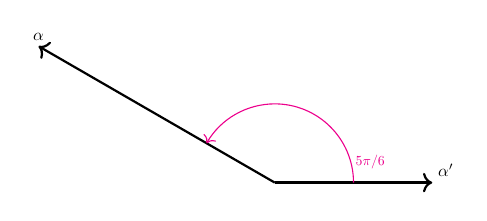
\begin{tikzpicture}

\draw[->,black!80!black,thick] (0,0) -- (0:2cm);
\draw[->,black!80!black,thick] (0,0) -- (150:3.464cm);
\draw[magenta,->](1,0) arc(0:150:1cm)node[pos=0.1,right,scale=0.5]{$5\pi/6$};
\node[anchor=south west,scale=0.6] at (2,0) {$\alpha'$};
\node[anchor=south,scale=0.6] at (-3, 1.732) {$\alpha$};
\end{tikzpicture}
\end{center}
By taking suitable $\bZ$-linear combinations, we can build more roots out of these simple roots:

\begin{center}
\begin{tikzpicture}
\foreach\ang in {60,120,...,360}{
 \draw[->,black!80!black,thick] (0,0) -- (\ang:2cm);
}
\foreach\ang in {30,90,...,330}{
 \draw[->,black!80!black,thick] (0,0) -- (\ang:3.464cm);
}
\draw[magenta,->](1,0) arc(0:150:1cm)node[pos=0.1,right,scale=0.5]{$5\pi/6$};
\node[anchor=south west,scale=0.6] at (2,0) {$\alpha'$};
\node[anchor=south,scale=0.6] at (-3, 1.732) {$\alpha$};
\node[anchor=south,scale=0.6] at (-1, 1.732) {$\alpha + \alpha'$};
\node[anchor=south,scale=0.6] at (1, 1.732) {$\alpha + 2 \alpha'$};
\node[anchor=south,scale=0.6] at (3, 1.732) {$\alpha + 3 \alpha'$};
\node[anchor=south,scale=0.6] at (0, 3.464) {$2\alpha + 3 \alpha'$};
\draw [dashed] (-6.464, 1.732) -- (6.464, -1.732);
\end{tikzpicture}
\end{center}
Recall that the only possible degrees between two root vectors are multiples of $\pi/6$, and no scaled vectors of given roots other than the vector and its opposite can appear as roots (reduced).
The ones above the dashed line (i.e. ones with names) are the chosen positive roots.
This gives the root space decomposition of $\frg_2$, where we can find the dimension of $\frg_2$ (hence Proposition \ref{prop:dim}) from this:
$$
\dim \frg_2 = \text{(rank)} + \text{(number of roots)} = 2 + 12 = 14.
$$
The highest root is $\beta_0 = 2 \alpha + 3 \alpha'$ (literally the ``highest'' one in the above diagram), and the Weyl group of $\frg_2$ is the symmetric group of a regular hexagon, which is the dihedral group of order 12.


\subsection{$G_2$ as a symmetry group of rolling balls}

Here we introduce an another definition of $G_2$, as a symmetry group of \emph{rolling balls}, discovered by Baez and Huerta \cite{baez2014g2}.
This section is not necessary for the upcoming discussions on modular forms\footnote{Maybe related? Who knows!}, but we include this because of its own interest.

We have a large ball of radius $R > 1$, and we are going to roll a unit ball around it, without slipping or twisting.
Then the corresponding configuration space is $\bS^2 \times \SO(3)$: $\bS^2$ for the point of contact and $\SO(3)$ for the rotation of the small ball.
Now, we define ``lines'' on the configuration space as paths along a great circle on the large ball, i.e. two points are connected if one can move the small ball from one state to the other state by rolling over a great circle (without slipping or twisting, of course).

Now, we consider another (incidence) geometry, comes from our one and only\footnote{Of course, there are two, but let's focus on the split one. Sorry for the non-split octonion...} octonion $\bO$.
The ``points'' are 1-dimensional \emph{null subalgebra} of $\Im(\bO)$: $p_x := \langle x \rangle \subset \Im(\bO)$ with $\rN(x) = 0$.
The ``lines'' are 2-dimensional null subalgebras spanned: i.e. two points $p_x = \langle x \rangle$ and $p_y = \langle y \rangle$ are connected if and only if $xy = 0 = yx$.
Then the group $G_2$ acts naturally on this space, which we denote as
$$
\mathbb{P}C = \{\langle x \rangle: 0 \ne x \in \Im(\bO), \rN(x) = 0\}.
$$
One can check that this space is isomorphic to
$$
\frac{\bS^2 \times \bS^3}{(a, b) \sim (-a, -b)} \simeq \mathbb{RP}^{2} \times \bS^3
$$
which is very close to the configuration space of the rolling ball, but not exactly.
To make them coincide, we can replace
\begin{itemize}
    \item small unit ball with \emph{spinor}: it needs to roll \emph{twice} to get back to the original position
    \item large ball with $\mathbb{RP}^{2}$: in other words, rolling a pair of spinor together in sync around the large ball.
\end{itemize}
Now we have the following amazing theorem.
\begin{theorem}[Baez--Huerta \cite{baez2014g2}]
    The symmetry group of a rolling spinor over $\mathbb{RP}^2$ is $G_2$ if and only if $R = 3$.
\end{theorem}
% \newpage
\section{Heisenberg parabolic subgroup and cubic rings}
\label{sec:g2heisenberg}

For $G_2$, we have a very special parabolic subgroup called \emph{Heisenberg parabolic subgroup}, which encode all information of Fourier coefficients of modular forms on $G_2$ (Section \ref{subsec:g2modfourier}).
Especially, the orbit of the character group under the adjoint action (of Levi component) is in bijection with the isomorphism classes of the \emph{cubic rings}, and these will parametrize Fourier coefficients of modualar forms on $G_2$.
Most of the discussions in the following can be found in Gan--Gross--Savin \cite{gan2002fourier}.


\subsection{Heisenberg parabolic subgroup of $G_2$}

Here $G_2$ is considered as an algebraic group over $\bZ$.
Recall that we have a bijection between (conjugacy classes of) parabolic subgroups as follows.
Let $G$ be a split group with a maximal (split) torus $T$ and a Borel subgroup $B$.
Let $J \subseteq \Delta$ be a subset and define $\Phi(J) := \bZ J \cap \Phi(G, T)$, where $\Phi(G, T)$ is the set of roots of $T \subset G$.
Then there exists a unique parabolic subgroup $P_J \supseteq B$ with a unipotent radical $U_J$ such that
$$
    \Lie U_J = \bigoplus_{\alpha \in \Phi^+ - (\Phi(J) \cap \Phi^+)} \frg_\alpha
$$
\begin{theorem}
We have a bijection
\begin{align*}
    \{ J \subseteq \Delta\} &\leftrightarrow \{\text{parabolic subgroups of }G \text{ containing }B\}     \\
    J &\mapsto P_J.
\end{align*}
\end{theorem}
This is an order-preserving bijection: we have $P_{\emptyset} = B$ and $P_{\Delta} = G$.
The Levi subgroup $L_J$ of $P_J$ is also equal to the subgroup of $G$ generated by the centralizer $C_G(T)$ and $G_\alpha$ for $\alpha \in J$.
See \cite[Theorem 1.9.2]{getz2023introduction} or Chapter 1.9 of loc. cit. for a general theory that covers quasi-split $G$.

Let's specialize it to the \emph{maximal} parabolic subgroups.
These subgroups correspond to the subset of $\Delta$ of the form $\theta = \Delta - \{\alpha\}$ for some $\alpha \in \Delta$.
The parabolic subgroup $P = P_\theta$ admits a Levi decomposition $P = LU$, where
$$
\Lie L = \Lie T \oplus \left(\bigoplus_{\beta: m_\alpha(\beta) = 0} \frg_\beta \right)
$$
where $m_\alpha(\beta)$ is the multiplicity of $\alpha$ in the root $\beta$.
The unipotent radical $U$ has a Lie algebra
$$
V = \Lie U = \bigoplus_{\beta: m_\alpha(\beta) > 0} \frg_\beta.
$$
It admits an action of the center $Z(L) \simeq \bG_m$, which gives a grading of $V$:
\begin{align*}
    V &= \bigoplus_{n \ge 1} V_n, \\
    V_n &= \bigoplus_{\beta: m_\alpha(\beta) = n} \frg_\beta.
\end{align*}
We have a canonical $L$-stable filtration of $U$, corresponds to the filtration of $V$: we have
$$
U = U_1 \supset U_2 \supset \cdots \supset U_d \supset \{1\}
$$
with $\Lie(U_i / U_{i+1}) = V_i$. The commutator on $U$ gives a map $U_i \times U_j \to U_{i+j}$, and this corresponds to the Lie bracket $V_i \times V_j \to V_{i+j}$ by passing to the quotients.

In our case, we first fix our set of simple roots $\Delta = \{\alpha, \alpha'\}$ above and have a corresponding Borel subgroup $B \subset G_2$.
We consider the maximal parabolic subgroup $P = LU$ associated with the subset $J = \Delta - \{\alpha\} = \{\alpha'\} \subset \Delta$.
Then
$$
\Phi^+ - (\Phi(J) \cap \Phi^+) = \{\alpha, \alpha + \alpha', \alpha + 2 \alpha', \alpha + 3 \alpha', \beta_0\}
$$
where the first four of them has $m_\alpha(-) = 1$ (contribute to $V_1$) and $m_\alpha(\beta_0) = 2$ (contribute to $V_2$).
The filtration of $U$ is
$$
U = U_1 \supset U_2 = U_{\beta_0} \supset \{1\}
$$
where $U_{\beta_0} = Z(U) = [U, U]$, and $U^{\mathrm{ab}} = U / [U, U] \simeq V_1$ has dimension 4.



\subsection{Cubic rings}

\label{subsec:cubicring}

The Levi subgroup $L$ acts on $U$ by conjugation, and this induces an action of $L$ on $\Hom(U, \bG_a) = \Hom(U^{\mathrm{ab}}, \bG_a)$.
We have the following description of the representation:
\begin{proposition}
\label{prop:repL}
The representation $L$ on the space $\Hom(U, \bG_a) = \Hom(U^\mathrm{ab} , \bG_a)$ is isomorphic to the twisted representation of $\GL_2$ on the space of binary cubic forms
$$
p(x, y) = ax^3 + bx^2 y + cxy^2 + dy^3
$$
defined as
$$
\begin{pmatrix}
    A & B \\ C & D
\end{pmatrix} \cdot p(x, y) = \frac{1}{\det(\gamma)} \cdot p(Ax + Cy, Bx + Dy), \quad \gamma = \begin{pmatrix}
    A & B \\ C & D
\end{pmatrix} \in \GL_2.
$$
\end{proposition}

Later, this space will serve as a parametrizing space of the Fourier coefficients of modular forms on $G_2$.
Proposition \ref{prop:repL} is even true over $\bZ$, and in fact, each orbit is in bijection with an isomorphism class of \emph{cubic rings}: a ring which is a free $\bZ$-module of rank 3.

\begin{proposition}[Delone--Fadeev \cite{delone1964theory}, Gan--Gross--Savin \cite{gan2002fourier}]
\label{prop:bcfcubic}
There is a bijection between the $\GL_2(\bZ)$-orbits of the space of binary cubic forms with integer coefficients and the set of isomorphism class of cubic rings.
This bijection preserves discriminants.
\end{proposition}
\begin{proof}
Here we only introduce the bijection without proof.
For a cubic ring $A$, we can always find a \emph{good basis} $(1, \alpha, \beta)$ so that $A = \bZ + \bZ \cdot \alpha + \bZ \cdot \beta$ and
$$
\begin{cases}
    \alpha \beta = -ad \\
    \alpha^2 = -ac + b \alpha - a \beta \\
    \beta^2 = -bd - d \alpha + c \beta
\end{cases}
$$
for $a, b, c, d \in \bZ$, and the corresponding binary cubic form is $f(x, y) = ax^3 + bx^2 y + cxy^2 + dy^3$.
Both $A$ and $f$ has the same discriminant
$$
    \Delta = b^2 c^2 + 18abcd - 4ac^3 - 4db^3 - 27 a^2 d^2.
$$
\end{proof}
For a binary cubic form $f(x, y) = ax^3 + bx^2 y + cx y^2 + dy^3$, we define it's \emph{content} simply as $e = \gcd(a, b, c, d)$.
Then the associated cubic ring $A$ can be written as $A = \bZ + e A_0$ for some other cubic ring $A_0$.
Especially, $f$ is primitive (i.e. the content is 1) if and only if the corresponding cubic ring is \emph{Gorenstein} (i.e. $\Hom(A, \bZ)$ is projective).
We also have a local variant of the content, namely $p$-depth for a prime $p$, which is the exponent of $p$ in the prime factorization of $e$.

% \newpage
\section{Local representation theory of $G_2$}
\label{sec:g2localrep}

\subsection{Archimedean}
\label{subsec:arch}

For a holomorphic modular form, the archimedean component of the associated automorphic representation is a \emph{holomorphic} discrete series.
For a general Lie group $G$ with a maximal compact subgroup $K$, \emph{when $G/K$ possesses a $G$-invariant holomorphic structure}, one can construct holomorphic discrete series using holomorphic line bundles on the homogeneous space $G/K$ (e.g. see \cite{schmid19762}).
One can try a similar construction of discrete series for $G_2(\bR)$, where it has a maximal compact subgroup $K = \SU_4 = (\SU_2 \times \SU_2) / \{\pm 1\}$.
Unfortunately, this does not work: we do not have a $G_2(\bR)$-invariant holomorphic structure on $G_2(\bR) / K$.
Instead, Gross and Wallach \cite{gross1996quaternionic} considered the ``next-best'' discrete series representation for $G_2(\bR)$:
\emph{quaternionic} discrete series representation.
These representations are constructed via $\rH^1$ of certain holomorphic line bundles on the ``twistor space covering'' $\mathscr{D} = G_2(\bR) / (L \cap K) \twoheadrightarrow G_2(\bR) / K$, which is a $\bP^1(\bC)$-bundle over $G_2(\bR) / K$.
These are parametrized by integers $k \ge 2$,\footnote{There are also \emph{limits} of discrete series representations when $k = 0$ and $1$, but we'll ignore these representations.} which have infinitesimal character $\rho + (k - 2) \beta_0$ where $\rho = \frac{1}{2}\sum_{\beta \in \Phi^+} \beta = 3 \alpha + 5 \alpha'$ is the Weyl root.
Its restriction to $K$ decomposes as
$$
(\pi_k)|_K \simeq \bigoplus_{n \ge 0} \Sym^{2k + n}(\bC^2) \boxtimes \Sym^n(\Sym^3 \bC^2),
$$
and the minimal $K$-type is the representation
$$
    \mathbb{V}_{k} := \Sym^{2k}(\bC^2) \boxtimes \mathbf{1} \quad \text{of }(\SU_2 \times \SU_2) / \{\pm 1\}
$$
of dimension $2k + 1$.
$\pi_k$ is a submodule of $\Ind_{P(\bR)}^{G_2(\bR)} \lambda_k$, where
$$
    \lambda_k = (\sgn)^k \cdot |\det|^{-k-1}.
$$

Recall that the adjoint representation of $L(\bR)$ on $\Hom(U(\bR), \bR)$ is isomorphic to the twisted representation of $\GL_2(\bR)$ on the space of binary cubic forms with coefficients in $\bR$ (Proposition \ref{prop:repL}).
We have $\Hom(U(\bR), \bR) \simeq \Hom(U(\bR), \bS^1)$ via $f \mapsto \chi = e^{2 \pi i f}$ (non-algebraic isomorphism), which takes the lattice $\Hom(U(\bZ), \bZ)$ to $\Hom(U(\bZ) \backslash U(\bR), \bS^1) = \{ \chi \in \Hom(U(\bR), \bS^1): \chi|_{U(\bZ)} = 1\}$.
The representation of $L(\bZ)$ on the later subgroup is isomorphic to twisted action of $\GL_2(\bZ)$ on the space of integral binary cubic forms.
Then a character $\chi$ is called \emph{generic} if the corresponding binary cubic form has nonzero discriminant (which we will denote as $\Delta(\chi)$).\footnote{Usually, a character $\psi: N(F) \to \bC^\times$ is called generic if it is nontrivial on each root (sub)group $N_\beta \le N$, and I think our definition also fits into this definition, but I haven't checked myself.}
Then the $L(\bR)$-action preserves sign of the discriminant, hence the set of generic characters break up into two orbits: those with $\Delta > 0$ (correponds to the real cubic algebra $\bR^3$) and those with $\Delta < 0$ (corresponds to the cubic algebra $\bR \times \bC$).
Wallach proved the following uniqueness result of Whittaker models of $\pi_k$ \cite{wallach2003generalized}:

\begin{proposition}
\label{prop:chihom}
    Let $\chi$ be a generic character of $U(\bR)$, and $k \ge 0$.
    Let
    $$
    \Wh_{k, \chi} = \Hom_{U(\bR)}(\pi_k, \chi) = \{\ell: \pi_k \to \bC, \ell(\pi_k(u)v) = \chi(u) \ell(v) \,\forall u \in U(\bR)\}
    $$
    be the space of $\chi$-Whittaker functionals on $\pi_k$. Then
    \begin{itemize}
        \item If $\Delta(\chi) < 0$, $\dim_{\bC} \Wh_{k, \chi} = 0$.
        \item If $\Delta(\chi) > 0$, $\dim_{\bC} \Wh_{k, \chi} = 1$, and it affords the representation $(\sgn)^k$ of $S_3 \simeq \stab(\chi) \subset \GL_2(\bR)$.
    \end{itemize}
\end{proposition}
The above result will be used to define \emph{Fourier coefficients} of modular forms on $G_2$ (Section \ref{subsec:g2modfourier}).

\subsection{Nonarchimedean}
\label{subsec:nonarch}

In Section \ref{subsec:gl2nonarch}, we studied (unramified) representations of $\GL_{2}(\bQ_p)$ and Hecke algebras.
A similar theory for $G_2$ is developed in \cite{gan2002fourier}, which we are going to introduce here.
Using this, we can describe the action of Hecke operators on $G_2$ modular forms on their Fourier coefficients (Section \ref{subsec:g2heckefourier}).

We have two fundamental representations of $G_2$: the 7-dimensional standard representation (corresponds to the embedding $G_2 \hookrightarrow \SO_7$ explained in \ref{subsec:g2def}), and the 14-dimensional adjoint representation.
Let $\chi_1$ and $\chi_2$ be the characters of these representations, respectively.
Then the representation ring $R(\what{G_2})$ of the dual group $\what{G_2} = G_2(\bC)$ (dual of $G_2$ is again $G_2$!) is a polynomial ring in $\chi_1$ and $\chi_2$, with highest weights $\lambda_1$ and $\lambda_2$ identified with coroots
\begin{align*}
    \lambda_1 &= \beta_0^\vee = (2\alpha + 3 \alpha')^\vee \\
    \lambda_2 &= (\alpha + 2 \alpha')^\vee.
\end{align*}
We have the following identities between $\chi_1$ and $\chi_2$:
$$
\begin{cases}
    \wedge^2 \chi_1 = \chi_1 + \chi_2 \\
    \wedge^3 \chi_1 = \chi_1^2 - \chi_2 \\
    \wedge^{7-n} \chi_1 = \wedge^n \chi_1.
\end{cases}
$$
For the spherical Hecke algebra $\cH_p(G_2):= C_c^\infty(G_2(\bZ_p) \backslash G_2(\bQ_p) / G_2(\bZ_p))$, Gross \cite{gross1998satake} computed Satake transform $\cS_{G_2}: \cH_p(G_2) \simeq R(\what{G_2})$ as
$$
\begin{cases}
    \varphi_1 = p^3 \chi_1 = \cS_{G_2}(K \lambda_1(p) K) + 1, \\
    \varphi_2 = p^5 \chi_2 = \cS_{G_2}(K \lambda_2(p) K) + p^4 + \varphi_1.
\end{cases}
$$


Using the equation above, we can find a decomposition of the double cosets $K \lambda_i(p) K$ into single $K$-cosets of the form $ulK$, where $u \in U(\bQ_p)$ and $l \in L(\bQ_p) \simeq \GL_2(\bQ_p)$, which will be used to compute the action of the corresponding Hecke operators on Fourier coefficients (Section \ref{subsec:g2heckefourier}).
We can use \emph{relative} Satake transform corresponds to the restriction map $R(\what{G_2}) \to R(\what{L})$, and this gives the number of distinct cosets in the decomposition of $K \lambda_i(p) K$ for each $l$.
More precisely, the relative Satake transform $\cS_{G_2 / L} : \cH_p(G_2) \to \cH_p(L)$ is defined as
$$
\cS_{G_2 / L}(c[t])(l) = |\delta_P(l)|^{1/2} \cdot \int_{U} c[t](lu) \dd u
$$
and it fits into the following commutative diagram
\begin{center}
\begin{tikzcd}
\cH_p(G_2) \arrow[r, "\cS_{G_2}"] \arrow[d, swap, "\cS_{G_2 / L}"]
& R(\what{G_2}(\bC)) \arrow[d, "\Res"] \\
\cH_p(L) \arrow[r, swap, "\cS_{L}"]
& R(\what{L}(\bC))
\end{tikzcd}
\end{center}

\begin{proposition}
\label{prop:relsat}
Fix $t \in G_2$ and $l \in L$.
Let $c[t] = \dso_{KtK} \in \cH_p(G_2, K)$ be the characteristic function.
Then
\begin{align*}
\cS_{G_2 / L}(c[t])(l) = |\delta_P(l)|^{1/2} \cdot \#\{ulK \subset KtK, u \in U\}
\end{align*}
\end{proposition}
Combining Proposition \ref{prop:relsat} with the restriction formula
\begin{align*}
    \Res(\chi_1) &= \det + \chi + 1 + \chi^\ast + \det{}^{-1} \\
    \Res(\chi_2) &= \Res(\chi_1) + \det \cdot \chi + \chi \cdot \chi^\ast + \det{}^{-1} \cdot \chi^\ast - 1,
\end{align*}
we can compute the number of distinct cosets of the form $ulK$ in $K\lambda_1(p)K$ and $K\lambda_2(p)K$ for given $l$ (Corollary 13.3 and 13.4 of \cite{gan2002fourier}).
One can find single cosets for each $l$ with carefully chosen $u$ match with the number: for example, we have the following result \cite[Proposition 14.2]{gan2002fourier}.

\begin{proposition}
Let $l$ lies in the double coset of either
$$
   \begin{pmatrix}
       p & \\ & p
   \end{pmatrix}, \quad
   \begin{pmatrix}
       p & \\ & 1
   \end{pmatrix}, \quad
   \begin{pmatrix}
       1 & \\ & p^{-1}
   \end{pmatrix}, \quad
   \begin{pmatrix}
       p^{-1} & \\ & p^{-1}
   \end{pmatrix}
$$
in $L \simeq \GL_2$, and $u$ lies in $U(\bZ_p)$, then $ulK$ is contained in the $K$-double coset of $\lambda_1(p)$ in $G$.
For such $l$, the representatives $u$ of the distinct right cosets of $U(\bZ_p) \cap l U(\bZ_p) l^{-1}$ in $U(\bZ_p)$ give the distinct right cosets of the form $ulK$ in $K \lambda_1(p) K$.
\end{proposition}
For other $l \in L$ and the double coset $K \lambda_2(p) K$, $u$ can be chosen as elements in certain root groups (See \cite[Section 14]{gan2002fourier} for details).

% \newpage
\section{Modular forms on $G_2$}
\label{sec:g2mod}

\subsection{Definition}
\label{subsec:g2moddef}

Fix the \emph{weight} $k \ge 2$ and a quaternionic discrete series representation $\pi_k$ of $G_2(\bR)$ introduced in Section \ref{subsec:arch}.
Let $\scA = \scA(G_2)$ be the space of automorphic forms on $G_2$: the are the functions on $G_2(\bA)$ which are
\begin{itemize}
    \item left $G_2(\bQ)$-invariant,
    \item right-invariant under some open compact group $K_f \subseteq G_2(\bA_\fin)$,
    \item annihilated by an ideal $J \subseteq \cZ(\frg_2)$ of finite codimension in the center $\cZ(\frg_2)$ of the universal enveloping algebra of $\frg_2 = \Lie G_2(\bR)$,
    \item has uniform moderate growth.
\end{itemize}
Note that the definition is slightly different from the literature, e.g. we are not assuming $K$-finiteness (compare this with the definition in Section \ref{subsec:gl2auto}).
More explanation can be found in \cite[Section 7]{gan2002fourier}.
Also, we are mainly interested in the modular forms of ``level 1'', i.e. when $K_f = G_2(\what{\bZ})$.

\begin{definition}
\label{def:g2mod}
The space of modular forms of weight $k$ and level 1 on $G_2$ is
$$
M_k(G_2) = \Hom_{G_2(\bR) \times G_2(\widehat{\bZ})} (\pi_k \otimes \bC, \scA),
$$
and the subspace of cusp forms is
$$
S_k(G_2) = \Hom_{G_2(\bR) \times G_2(\widehat{\bZ})} (\pi_k \otimes \bC, \scA_0).
$$
\end{definition}
By definition, $f \in M_k(G_2)$ is neither a function on $G_2(\bR)$ nor $G_2(\bA)$, but a $G_2(\bR) \times G_2(\what{\bZ})$-equivariant linear map from $\pi_k \otimes \bC$ to $\scA$.
Once you choose a vector $v \in \pi_k$, then $f(v)$ is indeed an automorphic form on $G_2$.
By the theorem of Harish-Chandra \cite[Theorem 1.7]{borel1979automorphic}, these spaces are finite dimensional.
Also, it admits an action of the spherical Hecke algebra
$$
\cH(G_2(\bA_\fin), G_2(\what{\bZ})) \simeq \what{\bigotimes_p} \,\cH_p(G_2)
$$
and the action on Fourier coefficients will be explained in Section \ref{subsec:g2heckefourier}.

\subsection{Fourier coefficients and expansion}
\label{subsec:g2modfourier}

% Let's recall the general theory of Whittaker--Fourier coefficients and the examples from classical \& Siegel modular forms.

Let $f \in M_k(G_2)$ and $v \in \pi_k$.
Then $f(v)$ can be viewed as a function on the double coset space
$$
G_2(\bQ) \backslash G_2(\bA) / G_2(\widehat{\bZ}) \simeq G_2(\bZ) \backslash G_2(\bR)
$$
where the homeomorphism comes from the strong approximation theorem.
For $\chi \in \Hom(U(\bZ) \backslash U(\bR), \bC^\times)$ define a linear functional $\ell_\chi$ on $\pi_k$ as
$$
\ell_\chi(v) = \int_{U(\bZ) \backslash U(\bR)} f(v)(u) \overline{\chi(u)} \dd u.
$$
Then $\ell_\chi \in \Wh_{k, \chi}$, and for $\gamma \in L(\bZ)$, $\ell_{\gamma \cdot \chi} = \gamma \cdot \ell_\chi$.
By Proposition \ref{prop:chihom}, $\ell_\chi = 0$ for $\Delta(\chi) < 0$, and $\ell_\chi$ lies in a 1-dimensional space if $\Delta(\chi) > 0$.
For the latter case, fix $\chi_0$ with $\Delta(\chi_0) > 0$ and a basis $l_0$ of $\Wh_{k, \chi_0}$.
There exists $g \in L(\bR)$ with $\chi = g \cdot \chi_0$, well defined up to the right multiplication by $\stab(\chi_0) \simeq S_3$.
The linear functional $\lambda_k(g) \cdot (g \cdot \ell_0)$ is a well-defined basis element of $\Wh_{k, \chi}$ (independent of the choice of $g$), hence
$$
\ell_\chi = c_\chi(f)\cdot \lambda_k(g) \cdot (g \cdot \ell_0)
$$
for some constant $c_\chi(f)$.
For \emph{even} $k$, $c_\chi(f)$ depends only on the $L(\bZ)$-orbit of $\chi$, and these orbits are indexed by (isomorphism classes of) cubic rings $A$ with $\disc(A) > 0$, so $A \otimes \bR \simeq \bR^3$.
We write $c_A(f)$ for the constants $c_\chi(f)$ and call it as $A$-th Fourier coefficient of $f$.
For \emph{odd} $k$, the situation is more subtle, since $c_\chi(f)$ depends on the $L(\bZ)$-orbit \emph{and} the orientation of $A$, i.e. the choice of a basis element $e$ of $\bigwedge^3 A \simeq \bZ$.
In this case, coefficients are only determined up to sign.

% We have a multiplicity one theorem for these Fourier coefficients: for $f \in M_k^0$, $c_A(f) = 0$ for all $A$ implies $f = 0$.
How much do Fourier coefficients $c_A(f)$ know about $f$ itself?
First of all, cusp forms are determined by the Fourier coefficients:
\begin{proposition}[Gan--Gross--Savin {\cite[Proposition 8.4]{gan2002fourier}}]
\label{prop:g2modmult1}
If $f \in S_k(G_2)$ satisfies $c_A(f) = 0$ for all cubic rings $A$, then $f = 0$.
\end{proposition}
% \begin{proof}
    
% \end{proof}
The proof in \cite{gan2002fourier} utilizes another maximal parabolic subgroup $Q = P_{\Delta - \{\alpha'\}} = P_{\{\alpha\}}$.
Also, we have the following analogue of \emph{Hecke bound} of Fourier coefficients for cusp forms:\footnote{I believe that this bound is not optimal - we may expect a smaller exponent possibly from Ramanujan conjecture (as in the case of modular forms).
Unfortunately, I have no idea what the optimal exponent would be.
Note that we expect generalized Ramanujan conjecture (temperedness of local factors $\pi_p$ of $\pi = \pi_f$) for $G_2$ \cite{sarnak2005notes}, but it is not clear how this could be related to the Fourier coefficients.}
\begin{proposition}[Gan--Gross--Savin {\cite[Proposition 8.6]{gan2002fourier}}]
\label{prop:g2heckebound}
    For $f \in S_k(G_2)$, there exists a constant $C_f > 0$ such that
    $$
        |c_A(f)| \le C_f \cdot |\disc(A)|^{(k+1)/2}
    $$
    for any totally real cubic ring $A$.
\end{proposition}

Recall that we have Fourier \emph{expansions} of holomorphic modular forms, where the basis elements are exponential functions.
Similarly, we have a Fourier expansion for Maass wave forms (i.e. non-holomorphic analogue of holomorphic modular forms), with the basis elements given by Bessel functions (see \cite[Section 1.9]{bump1998automorphic}).
Pollack developed a similar theory for all exceptional groups, including $G_2$, $F_4$, $E_6$, $E_7$, and $E_8$ \cite{pollack2020fourier}.
To do this, he considered the modular forms $f \in M_k(G_2)$ as the associated vector-valued functions $F = F_f : G_2(\bA) \to \bV_k^\vee$ via $F_f(g)(v) := f(v)(g)$.
Especially, he consider the restriction of $F$ onto the real points $G_2(\bR)$.
He proved that, for each character $\chi: U(\bZ) \backslash U(\bR) \to \bS^1$, there exist (vector-valued) basis functions $W_\chi$ on $G_2(\bR)$ are vector-valued functions which are given by solutions of \emph{Schmid operators}.
He solved the equations explicitly and expressed the solutions in terms of Bessel functions.
Before we state the result, note that we have a $\GL_2$-invariant symplectic form on $V_1(\bR) \simeq \det^{-1} \otimes \Sym^{3}(\bR^2)$, given by
$
\langle f, f' \rangle = ad' - \frac{1}{3} bc' + \frac{1}{3} cb' - da'
$
for $f = ax^3 + bx^2 y + cxy^2 + dy^3$ and $f' = a'x^3 + b'x^2 y + c' xy^2 + d'y^3$.
Now, we have the following theorem.

\begin{theorem}[Pollack \cite{pollack2020fourier,pollack2021modular}]
\label{thm:g2modfourierexp}
Let $F$ be a modular form on $G_2$ of weight $k$ and level 1, considered as a vector-valued function $F: G_2(\bR) \to \bV_k^\vee$.
Let
$$
F_0(g) = \int_{U_{\beta_0}(\bZ) \backslash U_{\beta_0}(\bR)} F(ng) \dd n
$$
be the constant term of $F$ along the center $U_{\beta_0} = Z(U)$ of the unipotent part of the Heisenberg parabolic subgroup.
% Let $V_1 = $
For $x \in V_1(\bR) \simeq \Lie(U(\bR)^{\mathrm{ab}})$ and $g \in L(\bR) \simeq \GL_2(\bR)$, $F_0$ has a Fourier expansion of the form
% there are complex numbers 
$$
F_0(\exp(x)g) = F_{00}(g) + \sum_{A} c_A(F) e^{-2 \pi i \langle f_A, x \rangle} W_{A}(g)
$$
where
\begin{itemize}
    \item The sum is over all cubic rings with $A \otimes \bR \simeq \bR^3$.
    \item $c_A(F)$ is the $A$-th Fourier coefficient of $F$.
    \item $f_A$ is the binary cubic form corresponds to $A$.
    \item $W_A : \GL_2(\bR) \to \bV_k^\vee$ is the basis function given by
    $$
        W_A(g) = \sum_{-k \le v \le k} W_{A, v}(g) \frac{x_\ell^{k + v}y_\ell^{k - v}}{(k+v)!(k-v)!}
    $$
    with $W_{A, v}: \GL_2(\bR) \to \bC$,
    $$
        W_{A, v}(g) = \det(g)^k |\det(g)| \left(\frac{|j(g, i) p_A(g \cdot i)|}{j(g, i) p_A(g \cdot i)}\right)^{v} K_v(|j(g, i)p_A(g \cdot i)|).
    $$
    Here $x_\ell, y_\ell$ are standard basis of weight vectors of the standard representation of $\SU_2$ (so that $\{x_\ell^{k + v} y_\ell^{k - v}\}_{-k \le v \le k}$ are a basis of $\bV_k$)\footnote{$\ell$ for \emph{long} root $\SU_2$.}, $p_A(z) = 2 \pi f_A(z, 1) =  2\pi(az^3 + bz^2 + cz + d)$ is the $2\pi$-multiple of the cubic polynomial corresponds to $A$, $j(g, i) = \det(g)^{-1}(ci + d)^3$ is the automorphy factor of $g = \left(\begin{smallmatrix}
        a & b \\ c & d
    \end{smallmatrix}\right)$, and $K_v(y) = \frac{1}{2}\int_0^\infty t^v e^{-y(\frac{t + t^{-1}}{2})} \frac{\dd t}{t}$ is the $v$-th Bessel function.
    % Note that $W_A = 0$ if $A \otimes \bR \simeq \bR \otimes \bC$, i.e. it is nonzero only if $A$ is a totally real cubic ring.
    \item $F^{00}$ is the constant term of $F^0$, which has a form of
    $$
        F_{00}(g) = \Phi(g) \frac{x_\ell^{2n}}{(2n)!} + \beta \frac{x_\ell^n y_\ell^n}{n! n!} + \Phi'(g) \frac{y_\ell^{2n}}{(2n)!}
    $$
    where $\beta \in \bC$ is a constant and $\Phi: L(\bR) \simeq \GL_2(\bR)\to \bC$ is associated with a holomorphic modular form of weight $3k$, and $\Phi'(g) = \Phi(g w_0)$ with $w_0 = \left(\begin{smallmatrix}
        -1 & 0 \\ 0 & 1
    \end{smallmatrix}\right)$.
    When $F \in S_k(G_2)$ is a cusp form, then this term vanishes.
\end{itemize}
\end{theorem}


\subsection{Hecke operators and Fourier coefficients}
\label{subsec:g2heckefourier}

For a holomorphic modular form $f = \sum_{n \ge 1} a_n(f) q^n \in S_k(\SL_2(\bZ))$, the Hecke operator $T_p$ acts on the coefficients via
$$
a_n(T_p f) = a_{np}(f) + p^{k-1} a_{n/p}(f),
$$
where $T_p$ is the Hecke operator corresponds to the characteristic function of $\GL_2(\bZ_p) \left(\begin{smallmatrix}
    p & \\ & 1
\end{smallmatrix}\right) \GL_2(\bZ_p)$ in the spherical Hecke algebra $\cH(\GL_2(\bQ_p), \GL_2(\bZ_p))$.
Gan--Gross--Savin \cite{gan2002fourier} gave a similar description for the modular forms on $G_2$, using the Hecke algebra structure and explicit coset decompositions in Section \ref{subsec:nonarch}.


\begin{proposition}[Gan--Gross--Savin {\cite[Proposition 15.6-15.8]{gan2002fourier}}]
Let $A$ be a cubic ring of $p$-depth zero, and for $i \ge 0$ define  $A_i := \bZ + p^i A$, which has $p$-depth $i$.
For $k$ even and $f \in M_k(G_2)$,
\begin{align*}
c_{A_i}(\chi_1 | f) &= p^{2k-1} c_{A_{i-1}}(f) + p^{k-1} \sum_{A_{i} \subset B \subset A_{i-1}} c_{B}(f) + c_{A_i} (f) \\
&\quad+ p^{-k} \sum_{A_{i+1} \subset B \subset A_{i}} c_{B}(f) + p^{1-2k} c_{A_{i+1}}(f) \qquad (i \ge 1),\\
c_{A}(\chi_1|f) &= p^{k-1} \sum_{A \subset_{p}B} c_B(f) + p^{-1}(n_A - 1) c_A(f) \\
&\quad+ p^{-k} \sum_{A_1 \subset B \subset A} c_B(f) + p^{1-2k} c_1(f), \\
c_{A_i}(\chi_2|f) &= c_{A_i}(\chi_1|f) + p^{3k-2} \sum_{A_{i-1} \subset B \subset A_{i-2}} c_B(f) + p^{-1} \sum_{A_{i+1} \subset C \subset A_{i-1}} c_C(f) \\
&\quad + p^{-1}c_{A_i}(f) + p^{1-3k} \sum_{A_{i+2} \subset B \subset A_{i+1}} c_B(f) \qquad (i \ge 2)
\end{align*}
where $n_A = \#\{B: A_1 \subset B \subset A\}$. For the last equation, each $C$ in the second sum is a ring with $C / A_{i+1} \simeq \bZ / p^2 \bZ$.
\end{proposition}
For example, when $A / pA$ is a field, the first equation simplifies as
$$
c_A(\chi_1 | f) = -\frac{1}{p} c_A(f) + p^{1-k} c_{A_1}(f).
$$
We\footnote{To be precise, they \cite{gan2002fourier} have, not me.} have a similar description of $c_{A}(\chi_2|f)$ and $c_{A_1}(\chi_2|f)$, but more complicated.
When $A / pA$ is a field, then \cite[Corollary 15.9]{gan2002fourier}
\begin{align*}
    c_A(\chi_2|f) &= \left(\frac{1}{p} + \frac{1}{p^2}\right) c_A(f) - p^{-2k} c_{A_1}(f) + p^{1-3k} \sum_{A_2 \subset B \subset A_1} c_B(f) \\
    c_{A_1}(\chi_2|f) &= -p^{2k - 2} c_{A}(f) + \left(1 + \frac{1}{p}\right) c_{A_1}(f) + p^{1-2k} c_{A_2}(f) \\
    &\quad + \sum_{A_3 \subset B \subset A_2} p^{1- 3k} c_B(f).
\end{align*}

When $f$ is a Hecke eigenform, we have a stronger result than Proposition \ref{prop:g2modmult1}.
\begin{theorem}[Gan--Gross--Savin {\cite[Theorem 16.2]{gan2002fourier}}]
Let $f \in M_k(G_2)$ be a Hecke eigenform.
If $c_A(f) = 0$ for all \emph{Gorenstein} rings, then all the Fourier coefficients of $f$ vanish.
In particular, if $f$ is a nonzero cuspidal Hecke eigenform, then $c_A(f) \ne 0$ for some Gorenstein ring $A$.
\end{theorem}
The analogous result is true for the holomorphic modular forms: if $f \in S_k(\Gamma_1)$ is a Hecke eigenform, then $a_1(f) \ne 0$.
This is because $a_n(f)$ is completely determined by $a_1(f)$ and the Hecke eigenvalues of $f$, and the above theorem is also proved with a similar argument.

\subsection{Examples}
\label{subsec:g2modex}

If we cannot find any single example of a nonzero modular form, then there's no reason to develop such a theory.
Here we introduce examples from \cite{gan2002fourier}: Eisenstein series and theta series.

Let $k \ge 2$ be an even integer.
Recall that we have an embedding (Section \ref{subsec:arch})
$$
i: \pi_{k} \hookrightarrow \Ind_{P(\bR)}^{G_2(\bR)} \lambda_{k}.
$$
The character $\lambda_k$ is the archimedean component of the global character
$$
\chi_k = |\det|^{-k-1} : P(\bA) \to \bC^\times
$$
which is unramified at all finite places.
Consider the induced representation
$$
I(k) = \Ind_{P(\bA)}^{G_2(\bA)} \chi_k = \bigotimes_v I_v(k).
$$
For each finite $p < \infty$, choose the unique normalized vector $\varphi_p^\circ \in I_p(k)$ fixed by $G_2(\bZ_p)$ and $\varphi_p^\circ(1) = 1$.
For $\varphi_\infty \in \pi_k$, let
$$
\varphi = i(\varphi_\infty) \otimes \left(\bigotimes_{p} \varphi_p^\circ\right) \in I(k)
$$
and form the Eisenstein series
$$
E({\varphi}, g) = \sum_{\gamma \in P(\bQ) \backslash G_2(\bQ)} {\varphi}(\gamma g).
$$
This converges absolutely when $k > 2$, and defines an element of $\cA$ right-invariant under $G_2(\what{\bZ})$.
Thus, we get a nonzero element
$$
E_k: \varphi_\infty \mapsto E(\varphi, g)
$$
in $M_k$.
Now, for each character $\chi : U(\bR) \to \bS^1$ trivial on $U(\bZ)$, we can consider it as a character on $U(\bA)$ trivial on $U(\bQ)$ and $U(\what{\bZ})$ (by strong approximation).
To compute the corresponding Fourier coefficients, one needs to observe
\begin{align*}
\ell_\chi(\varphi) &= \int_{U(\bQ) \backslash U(\bA)} E(u) \overline{\chi(u)} \dd u \\
&= \int_{U(\bQ) \backslash U(\bQ)} \left( \sum_{P_2(\bQ) \backslash G_2(\bQ)} \varphi(\gamma u)\right) \overline{\chi(u)} \dd u.
\end{align*}
The double coset space $P(\bQ) \backslash G_2(\bQ) / P(\bQ)$ has four representatives, say $w_0, w_1, w_2, w_3$, with
$$
P(\bQ) w_0 P(\bQ) = P(\bQ) w_0 U(\bQ)
$$
an open orbit $P$, and only this double coset contributes to the integral above.
Hence we get a factorizable integral
\begin{align*}
\ell_\chi(\varphi) &= \int_{U(\bA)} \varphi(w_0 u) \overline{\chi(u)} \dd u \\
&= \left(\int_{U(\bR)} \varphi_\infty(w_0 u_\infty) \dd u_\infty\right)\left(\prod_{p < \infty} \int_{U(\bQ_p)} \varphi_p^\circ(w_0 u_p) \overline{\chi(u_p)} \dd u_p\right).
\end{align*}
Jiang and Rallis \cite{jiang1997fourier} computed the non-archimedean factors above (under certain assumptions):
\begin{proposition}[{\cite[Theorem 2]{jiang1997fourier}}]
Assume $\chi$ corresponds to a maximal cubic ring $A$.
If $A \otimes \bQ_p$ is one of the following:
$$
\begin{cases}
    \bQ_p \times \bQ_p \times \bQ_p \\
    \bQ_p \times \bQ_{p^2} & p \ne 2\\
    \bQ_{p^3} & \bQ_p \text{ containing all cube roots of unity},
\end{cases}
$$
($\bQ_{p^m}$ is the unique unramified extension of $\bQ_p$ of degree $m$),
then
$$
\int_{U(\bQ_p)} \varphi_p^\circ( w_0 u_p) \overline{\chi(u_p)} \dd u_p = c_p \cdot \zeta_{A \otimes \bZ_p}(k),
$$
where $c_p$ is an explicit universal constant independent of $A$.
\end{proposition}
As a result, up to a constant, we have
$$
\ell_\chi(\varphi) = \zeta_A(k) \cdot \left(\int_{U(\bR)} \varphi_\infty(w_0 u_\infty) \overline{\chi(u_\infty)}\dd u_\infty\right)
$$
and it remains to compute the archimedean factor.
It defines a nonzero linear form
$$
\varphi_\infty \mapsto \int_{U(\bR)} \varphi_\infty(w_0 u_\infty) \overline{\chi(u_\infty)}\dd u_\infty
$$
in $\Hom_{U(\bR)}(I_\infty(k), \chi)$, but unfortunately, we do not know whether its restriction to $\pi_k$ is also nonzero or not.
If we assume that the restriction is also nonzero for some $\chi$ with $\Delta(\chi) > 0$ (recall Proposition \ref{prop:chihom} that the space of the Whittaker functional is zero if $\Delta(\chi) < 0$), then the restriction is nonzero for \emph{all} $\chi$ with $\Delta(\chi) > 0$, so is $c_A(E_k)$.
Now, fix $\chi_0$ that corresponds to the cubic form $f(x, y) = x^2 y + xy^2$, and let $\ell_0 = \ell_{\chi_0}$.
Choose any $g \in L(\bR) \simeq \GL_2(\bR)$ with $\chi = g \cdot \chi_0$.
% Then for $g \in L(\bR) \simeq \GL_2(\bR)$, we can show that
Then we can show that
$$
(g \cdot \ell_0)(\varphi) = \delta_P(g)^{(k-2)/3} \cdot \left(\int_{U(\bR)} \varphi_\infty(w_0 u_\infty) \overline{\chi(u_\infty)}\dd u_\infty\right)
$$
and using (...), $\delta_P = |\det|^{-3}$ and $|\det(g)|^2 = \Delta(g \cdot \chi_0) = \disc(A)$, we can conclude
$$
c_A(E_k) = \zeta_A(k) \cdot \disc(A)^{k - 1/2} = c \cdot \zeta_A(1 - k)
$$
for some constant $c$, where the last equality comes from the functional equation of $\zeta_A$.
Considering the Proposition \ref{prop:g2heckebound} and $\zeta_A(k) = O(1)$ (as $\disc(A) \to \infty$), one can conclude that $E_k$ is not a cusp form.

% Another example is a weight 4 exceptional theta series.
% There is an another example in \cite{gan2002fourier}, which is a theta series of weight $4$.
Gan, Gross, and Savin gave another example in \cite{gan2002fourier}, which are theta series of weight 4.
For a Gorenstein cubic ring $A$, $A$-th Fourier coefficients $N(A, J_E)$, $N(A, J_I)$ of these theta series $\theta_E$ and $\theta_I$ count the number of embeddings  of $A$ into certain Jordan structures $J_I$ and $J_E$ on the cubic Jordan algebra $J = H_3(\bO)$ of 3 by 3 Hermitian matrices over octonions.
Especially, the linear combination
$$
% \theta = 91 \theta_I + 600 \theta_E
N(A) = 91 N(A, J_I) + 600 N(A, J_E)
$$
is studied in \cite{gross1999commutative}, and Gan proved that the corresponding theta series
$$
\theta = 91 \theta_I + 600 \theta_E
$$
is a constant multiple of $E_4$ \cite{gan2000siegel}.
Gan and Gross proved the corresponding formula \cite[Theorem 3]{gross1999commutative}
$$
N(A) = 2^7 \cdot 3^3 \cdot 5^2 \cdot 7 \cdot 13 \cdot \zeta_A(-3),
$$
but without using the theory of $G_2$ modular forms.

Unfortunately, all the examples above are not cusp forms, and it is not clear whether nonzero cusp forms exist at all.
In fact, Dalal \cite{dalal2023counting} computed the dimension of the space of $G_2$ modular forms of weight $k \ge 3$, using Arthur's trace formula.
Especially, there exists a unique normalized nonzero cusp form of weights 9 and 11 respectively, and it is natural to ask if one can compute Fourier coefficients of the form.\footnote{The minimal weight $\ge 3$ with a nonzero cusp form is $k = 6$, but Pollack didn't prove/conjecture that the normalized form in $S_6(G_2)$ has integer Fourier coefficients. At least, we know algebraicity of the Fourier coefficients.}
Using the exceptional theta correspondences, Pollack \cite{pollack2022exceptional,pollack2024computation} proved that the coefficients of these forms are all integers and that all the coefficients $c_A(f)$ for cubic rings of the form $A \simeq \bZ \times B$ vanish.
More generally, he also proved that there exists a basis of $S_k(G_2)$ whose Fourier coefficients lie in $\bQ^{\mathrm{cyc}} = \bQ(\mu_\infty)$, for $k \ge 6$\footnote{During the seminar talk, I explained this as an ``interesting'' fact, especially because the ``coefficient field'' is always abelian. Note that the coefficient fields of classical modular forms can be non-abelian (examples can be found in LMFDB), but only when \emph{we increase the levels}. If we keep the level as 1, then the coefficient field is just $\bQ$ (generated by Eisenstein series $E_4$ and $E_6$). Hence, we might even expect that the coefficient field of any $G_2$-modular form of level 1 is in a (abelian) number field, or even $\bQ$.}.
Note that a similar algebraicity result is known for holomorphic modular forms (if $f$ is a normalized Hecke eigenform, then its coefficient lies in a certain number field $K = K_f$).

% \newpage
\section{Further remarks}
\label{sec:further}

I end this note by introducing other works relevant to modular forms on $G_2$, which I don't have enough space (and knowledge) to write down the details.

\begin{itemize}
    \item We have a theory of (standard) $L$-functions for $G_2$ modular forms, especially their Rankin--Selberg type integral representations, developed by Gurevich--Segal \cite{gurevich2015rankin} and \c{C}i\c{c}ek et. al. \cite{cicek2022completed}.
    Especially, we have functional equations and Dirichlet series representations.
    \item There's an analogue of half-integral weight modular forms for $G_2$ by Leslie and Pollack \cite{leslie2024modular}, as automorphic forms on the double cover of $G_2$.
    Especially, they construct a modular form of weight $\frac{1}{2}$ on $G_2$, whose Fourier coefficients measure the size of 2-torsions of the narrow class groups.
    \item There are four other exceptional groups $F_4, E_6, E_7, E_8$, and we can define the notion of modular forms on these groups, too.
    In fact, there is a more uniform way to treat all five exceptional groups at once, via Jordan algebra and Freudenthal construction.
    This is well explained in an aribitrary paper of Pollack, e.g. \cite{pollack2020fourier}.
    \item Somehow, reductive groups of type $D_4$ also behave like exceptional groups.
    Weissman developed a similar theory of $D_4$ modular forms (to be precise, modular forms on $\Spin(4, 4)$ and $\Spin(8)$), including Fourier coefficients, local representation theory, and exceptional theta correspondences \cite{weissman2006d}.
    Interestingly, the Fourier coefficients of the $D_4$ modular forms are parameterized via Bhargava's cube \cite{bhargava2004higherI}.
    \item
    Gross and Lucianovic \cite{lucianovic2003quaternion,gross1996quaternionic} proved that there is a one-to-one correspondence between the space of \emph{ternary quadratic forms} and the \emph{quaternion algebras}, hence Fourier coefficients of genus 3 Siegel modular forms are parametrized by quaternion algebras.
    One of the main example comes from Kim's exceptional Eisenstein series on $E_7$ \cite{kim1992exceptional}, whose restriction on the Siegel upper half plane gives a weight 4 Siegel modular form with Fourier coefficients counding the number of embeddings of quaternion algebras into the Coxeter's order inside the non-split octonion.
    The \emph{anisotropic/compact} $G_2^a$ form a reductive dual pair with $\GSp_{6}$ in $E_8$,  and Volpato \cite{volpato2008some} proved that the lift of the constant function on $G_2^a$ coincides with the Siegel modular form mentioned above.
    
\end{itemize}

\newpage








% --- Bibliography ---

% Start a bibliography with one item.
% Citation example: "\cite{williams}".

\bibliographystyle{acm} % We choose the "plain" reference style
\bibliography{refs} % Entries are in the refs.bib file


% \begin{thebibliography}{1}

% \bibitem{williams}
%    Williams, David.
%    \textit{Probability with Martingales}.
%    Cambridge University Press, 1991.
%    Print.

% % Uncomment the following lines to include a webpage
% % \bibitem{webpage1}
% %   LastName, FirstName. ``Webpage Title''.
% %   WebsiteName, OrganizationName.
% %   Online; accessed Month Date, Year.\\
% %   \texttt{www.URLhere.com}

% \end{thebibliography}

% --- Document ends here ---

\end{document}